\documentclass[pdf]{beamer}
%\mode<presentation>{}

\usepackage{amssymb,amsmath,amsthm,enumerate,mathtools}
\usepackage[utf8]{inputenc}
\usepackage{array}
\newcolumntype{C}[1]{>{\centering\arraybackslash}m{#1}}

\usepackage[parfill]{parskip}
\usepackage{graphicx}
\usepackage{caption}
\captionsetup[figure]{labelformat=empty}
\usepackage{subcaption}
\usepackage{bm}
\usepackage{amsfonts,amscd}
%\usepackage{gensymb}
\usepackage[]{units}
\usepackage{listings}
\usepackage{multicol}
\usepackage{tcolorbox}
\usepackage{physics}
\usepackage{multirow}
\usepackage{pgfplots,tikz}
\pgfplotsset{compat=1.7}
\usepackage{hyperref}
\hypersetup{
    colorlinks=true,
    linkcolor=franklinblue,
    filecolor=magenta,      
    urlcolor=cyan,
    bookmarks=true,
    citecolor= black
    % pdftitle={Overleaf Example},
    % pdfpagemode=FullScreen,
    }
\usepackage{colortbl}
\usepackage{booktabs}
\usepackage{gensymb}
\usepackage{color}
\usepackage{natbib}

\usepackage{tikz}
\usepackage{fixltx2e}
\usepackage[english]{babel}
\usepackage[absolute,overlay]{textpos}
%\usepackage{gnuplottex} % For t-distribution using gnuplot.
%The following function is use in students t distribution. 
% \def\basefunc{    gamma((\n+1)/2.)/(sqrt(\n*pi)*gamma(\n/2.))*((1+(x*x)/\n)^(-(\n+1)/2.))}    
% \def\n{7}
%\usepackage{tkz-fct} % For t-distribution plotting.
% \usepackage{pst-func} % For t-distribution plotting.
\usepackage{longtable}
\usepackage{changepage} 

\usetikzlibrary{shapes,decorations,arrows,calc,arrows.meta,fit,positioning}
\tikzset{
    -Latex,auto,node distance =1 cm and 1 cm,semithick,
    state/.style ={ellipse, draw, minimum width = 0.7 cm},
    point/.style = {circle, draw, inner sep=0.04cm,fill,node contents={}},
    bidirected/.style={Latex-Latex,dashed},
    el/.style = {inner sep=2pt, align=left, sloped}
}

%Normal Distribution
\pgfmathdeclarefunction{gauss_}{2}{\pgfmathparse{1/(#2*sqrt(2*pi))*exp(-((x-#1)^2)/(2*#2^2))}%
}
%Gamma Distribution
\pgfmathdeclarefunction{gammaPDF}{2}{
\pgfmathparse{1/(#2^#1*gamma(#1))*x^(#1-1)*exp(-x/#2)}
}

%%%%% For https://tikz.net/gaussians/ %%%%%

\usepackage{amsmath} % for \dfrac
\usepackage{tikz}
\tikzset{>=latex} % for LaTeX arrow head
\usepackage{pgfplots} % for the axis environment
\usepackage{xcolor}
\usepackage[outline]{contour} % halo around text
\contourlength{1.2pt}
\usetikzlibrary{positioning,calc}
\usetikzlibrary{backgrounds}% required for 'inner frame sep'
%\usepackage{adjustbox} % add whitespace (trim)

% define gaussian pdf and cdf
\pgfmathdeclarefunction{gauss}{3}{%
  \pgfmathparse{1/(#3*sqrt(2*pi))*exp(-((#1-#2)^2)/(2*#3^2))}%
}
\pgfmathdeclarefunction{cdf}{3}{%
  \pgfmathparse{1/(1+exp(-0.07056*((#1-#2)/#3)^3 - 1.5976*(#1-#2)/#3))}%
}
\pgfmathdeclarefunction{fq}{3}{%
  \pgfmathparse{1/(sqrt(2*pi*#1))*exp(-(sqrt(#1)-#2/#3)^2/2)}%
}
\pgfmathdeclarefunction{fq0}{1}{%
  \pgfmathparse{1/(sqrt(2*pi*#1))*exp(-#1/2))}%
}

\colorlet{mydarkblue}{blue!30!black}

% to fill an area under function
\usepgfplotslibrary{fillbetween}
\usetikzlibrary{patterns}
\pgfplotsset{compat=1.12} % TikZ coordinates <-> axes coordinates
% https://tex.stackexchange.com/questions/240642/add-vertical-line-of-equation-x-2-and-shade-a-region-in-graph-by-pgfplots

% plot aspect ratio
%\def\axisdefaultwidth{8cm}
%\def\axisdefaultheight{6cm}

% number of sample points
\def\N{50}

%%%%% End for https://tikz.net/gaussians/ %%%%%

\setbeamertemplate{caption}[numbered]

%new commands
\newcommand{\der}[2]{\frac{d#1}{d#2}}
\newcommand{\nder}[3]{\frac{d^#1 #2}{d #3 ^ #1}}
\newcommand{\pder}[2]{\frac{\partial #1}{\partial #2}}
\newcommand{\npder}[3]{\frac{\partial ^#1 #2}{\partial #3^#1}}
\newcommand{\sentencelist}{def}
\newcommand{\overbar}[1]{\mkern 1.5mu\overline{\mkern-1.5mu#1\mkern-1.5mu}\mkern 1.5mu}
\newcommand{\lined}{\overbar}
\newcommand{\perm}[2]{{}^{#1}\!P_{#2}}
\newcommand{\comb}[2]{{}^{#1}C_{#2}}
\newcommand{\intall}{\int_{-\infty}^{\infty}}
\newcommand{\Var}[1]{\text{Var}\left(#1\right)}
\newcommand{\E}[1]{\text{E}\left(#1\right)}
\newcommand{\define}{\equiv}
\newcommand{\diff}[1]{\mathrm{d}#1}
\newcommand{\empy}[1]{{\color{cadetblue}\texttt{#1}}}
\newcommand{\empr}[1]{{\color{franklinblue}\textbf{#1}}}
%https://tex.stackexchange.com/questions/192358/quickly-changing-all-the-file-paths-in-a-tex-file
%\newcommand{\pathtopdf}{C:/Users/bkwei/OneDrive - Franklin University/Desktop/Math_215/Data/IMDB/Processed} - Not Tested!
\newcolumntype{L}[1]{>{\raggedright\let\newline\\\arraybackslash\hspace{0pt}}m{#1}}
\newcolumntype{C}[1]{>{\centering\let\newline\\\arraybackslash\hspace{0pt}}m{#1}}
\newcolumntype{R}[1]{>{\raggedleft\let\newline\\\arraybackslash\hspace{0pt}}m{#1}}

\theoremstyle{remark}
\newtheorem*{remark}{Remark}
\theoremstyle{definition}

\newcommand{\examplebox}[2]{
\begin{tcolorbox}[colframe=darkcardinal,colback=boxgray,title=#1]
\end{tcolorbox}}

\newcommand{\eld}[1]{\frac{d}{dt}(\frac{\partial L}{\partial \dot #1}) - \frac{\partial L}{\partial #1}=0}
\newcommand{\euler}[1]{\frac{\partial L}{\partial #1}-\frac{d}{dt}(\frac{\partial L}{\partial \dot #1})}
\newcommand{\eulerg}[1]{\frac{\partial g}{\partial #1}-\frac{d}{dt}(\frac{\partial g}{\partial \dot #1})}
\newcommand{\divg}[1]{\nabla\cdot #1}
\newcommand{\prob}[1]{P(#1\vert I)}

\AtBeginSection[]{
  \begin{frame}
  \vfill
  \centering
  \begin{beamercolorbox}[sep=8pt,center,%shadow=true,
  rounded=true]{section}
    \LARGE
    \usebeamerfont{section}
    %\usebeamercolor[fg]{section}\inserttitle %\insertsectionhead\par%
    \setbeamercolor{section}{fg=white,bg=white}\insertsectionhead\par%
  \end{beamercolorbox}
  \vfill
  \end{frame}
}

\usetheme{Franklin} 
\def \i  {\item}
\def \ai {\item[] \quad \arrowbullet}
\newcommand \si[1]{\item[] \quad \bulletcolor{#1}}
\def \wi {\item[] \quad $\ \phantom{\Rightarrow}\ $}
\def \bi {\begin{itemize}\item}
\def \ei {\end{itemize}}
\def \be {\begin{equation*}}
\def \ee {\end{equation*}}
\def \bie {$\displaystyle{}
\def \eie {{\ }$}}
\def \bsie {\small$\displaystyle{}
\def \esie {{\ }$}\normalsize\selectfont}
\def \bse {\small\begin{equation*}}
\def \ese {\end{equation*}\normalsize}
\def \bfe {\footnotesize\begin{equation*}}
\def \efe {\end{equation*}\normalsize}
\renewcommand \le[1] {\\ \medskip \lefteqn{\hspace{1cm}#1} \medskip}
\def \bex {\begin{example}}
\def \eex {\end{example}}
\def \bfig {\begin{figure}}
\def \efig {\end{figure}}
\def \btheo {\begin{theorem}}
\def \etheo {\end{theorem}}
\def \bc {\begin{columns}}
\def \ec {\end{columns}}
\def \btab {\begin{tabbing}}
\def \etab {\end{tabbing}\svneg\svneg}
\newcommand \col[1]{\column{#1\linewidth}}
\def\vneg  {\vspace{-5mm}}
\def\lvneg {\vspace{-10mm}}
\def\svneg {\vspace{-2mm}}
\def\tvneg {\vspace{-1mm}}
\def\vpos  {\vspace{5mm}}
\def\lvpos {\vspace{10mm}}
\def\svpos {\vspace{2mm}}
\def\tvpos {\vspace{1mm}}
\def\hneg  {\hspace{-5mm}}
\def\lhneg {\hspace{-10mm}}
\def\shneg {\hspace{-2mm}}
\def\thneg {\hspace{-1mm}}
\def\hpos  {\hspace{5mm}}
\def\lhpos {\hspace{10mm}}
\def\shpos {\hspace{2mm}}

\logo{
\includegraphics[height=0.4in]{./style_files_franklin/FranklinUniversity_TM1.jpg}}

\title{BUSA 603}
\subtitle{Module 1:   Marketing Principles, Practices \& Metrics}

\beamertemplatenavigationsymbolsempty

\begin{document}

\author[B. Weikel, Franklin University]{
	\begin{tabular}{c} 
	\Large
	Brian Weikel\\
    \footnotesize \href{mailto:brian.weikel@franklin.edu}{brian.weikel@franklin.edu}
    \vspace{1ex}
\end{tabular}
\vspace{-4ex}}

\institute{
	
\includegraphics[height=0.4in]{./style_files_franklin/FranklinUniversity_TM1.jpg}\\
	Business Analytics\\
	Franklin University}

\date{Spring 2024}%{\today}

\begin{noheadline}
\begin{frame}[t]\maketitle\end{frame}
\end{noheadline}

\begin{frame}[t]{Outline\footnote{
These lecture notes map to chapters 1 and 12 of \cite{davis2022}.}}
\begin{enumerate}
\item Defining Marketing Analytics
\vspace{2.0ex}
\item Data, Analytics and Visualization 
\vspace{2.0ex}
\item A Marketing Metric Example
\vspace{2.0ex}
\item Marketing Analytics Strategy and Metrics
\vspace{2.0ex}
\item Strategic Marketing Analytics
\vspace{2.0ex}
\item Appendix
\end{enumerate}
\end{frame}

\section{Defining Marketing Analytics}

\begin{frame}[t]{What is Marketing?}
To succeed businesses in highly integrated and complex market economies require an understanding of \empr{marketing}.  \\
\vspace{1.5ex}
%\small
\begin{itemize}
\item Long-term business success is dependent on meeting consumer demand. Businesses which do not create value for their customers cannot expect to achieve long-term success.  
\item Marketing is a vital component to long-term success. 
\end{itemize}
\normalsize
\vspace{0.0ex}
Trying to define marketing simply is a difficult task. Wide debates have taken place in the marketing field over attempts to create an accepted definition of marketing.\footnote{See for example \cite{sheth2007} and \cite{zinkhan2007}.} 
\vspace{1.5ex}
\end{frame}


\begin{frame}[t]{Marketing Definitions Galore!}
Three such definitions of marketing, among many, highlight the inconsistencies in attempts to define it. \\
  \vspace{1.5ex}
\begin{enumerate}
  \item The process or technique of promoting, selling, and distributing a product or service.\footnote{``marketing.'' Merriam-Webster.com. Merriam-Webster, 2022. Web. 19 November 2022.}
  \item The process by which companies create value for customers and build strong customer relationships to capture value from customers in return (\cite{kotler2012}).
  \item The activity, set of institutions, and processes for creating, communicating, delivering, and exchanging offerings that have value for customers, clients, partners, and society at large.\footnote{\href{https://www.ama.org/the-definition-of-marketing-what-is-marketing/}{American Marketing Association (AMA), 2017}}
\end{enumerate}
\end{frame}

\begin{frame}[t]{Any of the Three Definitions Will be Sufficient}
As the three definitions above highlight, there is no accepted definition of marketing; rather definitions found across dictionaries, scholarly publications and marketing association materials are vague, contradictory, and sometimes both. \\
\vspace{1.5ex}
Despite this bewildering array of definitions, for this class any of the above definitions will be sufficient.
\end{frame}

\begin{frame}[t]{The ``4 P's''}
The term \empr{marketing mix} was developed by Neil Borden in 1949. ``An executive is a mixer of ingredients, who sometimes follows a recipe as he goes along, sometimes adapts a recipe to the ingredients immediately available, and sometimes experiments with or invents ingredients no one else has tried.'' \\
\vspace{1.5ex}
Edmund Jerome McCarthy proposed the concept of the marketing mix \empr{``4 P's''} in 1960, and modified it slightly in 1964.\footnote{For additional information see \cite{mccarthy1964}.} 
\begin{enumerate}
  \item Value creation via \empr{product}. A product refers to an item that satisfies the consumer's needs or wants.
  \item Value capture via \empr{price}.  Price is the only variable that has implications for revenue.
  \item Value delivery via \empr{place}.  Refers to providing customer access. 
\end{enumerate}
\end{frame}

\begin{frame}[t]{Extending the ``P's''}
\begin{enumerate}
  \setcounter{enumi}{3}
  \item Value communication via \empr{promotion}. May comprise elements such as advertising, public relations, direct marketing, and sales promotion.
\end{enumerate}
\cite{booms1981} expanded the set of P's by three. \\
\vspace{1.5ex}
\begin{enumerate}
\setcounter{enumi}{4}
\item \empr{People}.  Human factors who participate in service delivery; for example, interactions between employees and customers.
\item \empr{Physical evidence}. The environment in which service occurs, such as tangible commodities that facilitate service. 
\item \empr{Processes}.   The procedures, mechanisms, and flow of activities by which service and goods are delivered.
\end{enumerate}
\end{frame}

\begin{frame}[t]{What is Marketing Analytics?}
\empr{Marketing analytics} is the use of data to maximize marketing outcomes. Marketing analytics specifies the information needed for decision making and links the information to actionable decisions.\\ 
\vspace{1.5ex}
As of 2020 it had been estimated that more than \href{https://us.sganalytics.com/blog/2-5-quintillion-bytes-of-data-generated-everyday-top-data-science-trends-2020/}{2.5 quintillion bytes} of data are created each day.  \\ 
\vspace{1.5ex}
Marketing analytics is a growing field due to previously unimaginable amounts and quality of
data that are available with relatively few people to explore them. \\
\vspace{1.5ex}
\begin{tcolorbox}[colback=white!5,colframe=franklinblue]%,title=A nice heading]
There are a lot of small data problems that occur in big data.  They don't disappear because you've got lots of stuff.  They get worse. - David J. Spiegelhalter.
\end{tcolorbox}
\end{frame}

\begin{frame}[t]{Marketing Analytics Supports Marketing Priorities}
In a recent IBM global survey, over 700 chief marketing officers revealed their top priorities for marketing. \\ 
\vspace{1.5ex}
\begin{enumerate}
\item Embrace creative destruction. 
\begin{itemize}
\item This means adopting strategies of disruption.  
\item For example, \href{https://www.tiktok.com/about?lang=en}{Tiktok} in the social media space.
\end{itemize}
\item Enrich the arch of engagement. 
\begin{itemize}
\item This means finding new ways to engage new and old customers.  
\item Such as the \href{https://adage.com/article/marketing-news-strategy/victorias-secret-continues-rebrand-new-global-push/2437276}{rebranding of Victoria's Secret}, which is based in Columbus, Ohio.
\end{itemize}
\end{enumerate}
\end{frame}

\begin{frame}[t]{Continuing Education is Paramount}
\begin{enumerate}
  \setcounter{enumi}{2}
\item Inject data-driven insights into every corporate decision, which obviously includes  marketing decisions.  As discussed in this \href{https://hbr.org/2020/02/10-steps-to-creating-a-data-driven-culture}{Harvard Business Review article} (\cite{waller2020}), creating a data-driven culture is not as easy as it would seem.
\item Increase digital acumen. 
\begin{itemize}
\item This means pursuing a deeper understanding of marketing decisions through data and technology.  
\item Such as \href{https://ai.facebook.com/tools/\#frameworks-and-tools}{Meta AI capabilities}, \href{https://www.facebook.com/business/m/one-sheeters/conversion-lift}{Facebook Conversion Lift}, \href{https://skillshop.exceedlms.com/student/catalog/browse}{Google Skillshop}, and \href{https://www.ama.org/certifications/}{American Marketing Association certifications}.
\end{itemize}
% https://aws.amazon.com/training/learn-about/data-analytics/?th=tile&tile=learnabout
\end{enumerate}
\end{frame}

\section{Data, Analytics and Visualization}

\begin{frame}[t]{Primary and Secondary Data}
The three primary components of marketing analytics are \underline{data}, \underline{analytics} and \underline{visualization}. \\
\vspace{1.5ex}
Types of data. \\
\vspace{0.5ex}
\small
\begin{itemize}
\item \empr{Primary data} are collected especially to address a specific research objective.  Examples include, survey data, customer feedback, and data resulting from experimental designs.
\item \empr{Secondary data} were collected for some purpose other than solving the present problem.  For example, U.S. census data, \underline{syndicated} \underline{data} (such as sales, distribution, promotional \ldots metrics) as available from \href{https://www.iriworldwide.com/en-us}{IRI}, \href{https://nielseniq.com/global/en/}{NielsenIQ}, \href{https://www.npd.com/}{NPD}, and \href{https://www.spins.com/}{Spins}, and primary data collected previously.\footnote{Syndicated data is a type of aggregated data that brings together product retail sales activity across a particular set of parameters.  IRI and NPD have come together to form \href{https://www.circana.com/}{Circana}.} Secondary data at times has advantages to primary data:  cost (e.g., cost of internet search is small), time, and potentially accuracy. 
\end{itemize}
\end{frame}

\begin{frame}[t]{Steps for Using Data for Marketing Analytics}
\begin{description}
 \item [(1) Data Collection]
 \vspace{1.5ex}
 \item [(2) Data Storage and Management]
 \vspace{1.5ex}
 \item [(3) Data Cleaning] 
 \vspace{1.5ex}
 \item [(4) Data Structuring]
 \vspace{1.5ex}
 \item [(5) Data Integration]
 \vspace{1.5ex}
 \item [(6) Data Analysis]
 \vspace{1.5ex}
 \item [(7) Data Visualization]
 \vspace{1.5ex}
\end{description}
\end{frame}

\begin{frame}[t]{(1) Data Collection}
Always obtain the right data so the business questions of interest may be addressed. For brand engagement, detailed information about user interactions within their own website, social media, and other digital platforms would be useful.  For web analytics this may include, but is not limited to, time spent on website, and click and conversion rates. \\
\vspace{1.5ex}
For the \underline{service} metric \empr{return on marketing investment} (ROMI), which is incremental revenue due to marketing efforts multiplied by contribution margin divided by marketing expenditure, ensure you collect the \textit{proper} revenue, margin per unit or margin percents, and cost information.\footnote{An excellent reference on metrics used in marketing is \cite{bendle2020}.  For \empr{return on ad spend} (ROAS), margin per unit and margin percents are not needed.}  
\end{frame}

\begin{frame}[t]{(2) Data Storage and Management}
After data is collected, it must be stored and managed.  \\
\vspace{1.5ex} 
Data storage and management platforms include \href{https://aws.amazon.com/rds/aurora/}{Amazon Aurora}, \href{https://aws.amazon.com/rds/}{Amazon Relational Database Service} (RDS), \href{https://www.ibm.com/products/db2}{IBM Db2}, \href{https://www.microsoft.com/en-us/sql-server/sql-server-downloads}{Microsoft SQL Server}, \href{https://www.mongodb.com/atlas/database}{MongoDB}, \href{https://dev.mysql.com/}{MySQL}, \href{https://www.oracle.com/database/}{Oracle}, \href{https://www.sap.com/sea/products/technology-platform/hana.html}{SAP Hana Cloud}, \href{https://www.snowflake.com/en/}{SnowFlake}, and \href{https://www.teradata.com/}{Teradata}.  \\
\vspace{1.5ex}
In a pinch, \href{https://aws.amazon.com/s3/}{Amazon S3} buckets along with \href{https://aws.amazon.com/s3/features/access-points/}{S3 Access Points} can be organized to store and manage data.  \\
\vspace{1.5ex}
As data has become larger and at times less structured, the demand for cost-effective data storage solutions keeps increasing. \\ 
\end{frame}

\begin{frame}{Storing Data Securely}
\empr{Data security} is the practice of protecting digital information from unauthorized access, corruption, or theft throughout its entire life-cycle. \\
\vspace{1.5ex}
It is a concept that encompasses every aspect of information security from the physical security of hardware and storage devices to administrative and access controls, as well as the logical security of software applications. \\
\vspace{1.5ex}
It also includes organizational policies and procedures. \\
\vspace{1.5ex}
When properly implemented, robust data security strategies will protect an organization's information assets against cyber-criminal activities.  In addition, they will also guard against insider threats and human error, which remains among the leading causes of data breaches today. 
\end{frame}


\begin{frame}[t]{(3) Data Cleaning}
Cleaning involves dealing with data that are \underline{incomplete}, have \underline{outliers}, or is \underline{inconsistent}. When data are incomplete, it is necessary to deal with those records that have missing values. There are many ways to deal with missing values.\footnote{Imputation methods based on statistical technique include mean, hot-deck and multiple imputation.  Imputation via machine learning techniques include the use of deep learning, self-organizing maps, and k-nearest neighbor. For an introduction to missing data mechanisms and handling missingness see \cite{jakobsen2017}.}\\
\vspace{1.5ex} 
Cleaning also means identifying outliers in the data. Outliers are data values outside the range of typical values. \\
\vspace{1.5ex} 
Inconsistent data also needs to be cleaned. Inconsistent data means they do not make sense given variable definitions.
\end{frame}

\begin{frame}[t]{(4) Data Structuring}
Unstructured data do not reside in traditional databases and data warehouses. They may have some kind of internal structure (e.g., product reviewer and posting), but this pattern does not fit a relational data model. A \empr{relational data model} means data are stored in formally described tables so that tables can easily be related to one another.\\
\vspace{1.5ex} 
Data structuring is tied closely to data storage and management, and data cleaning. \\
\vspace{1.5ex} 
It is important to structure these data by organizing them in whatever format is best for analysis needs. Sometimes there is a trade-off between efficiency and organization.\footnote{For example, big data accessed real-time may need to be processed quickly. It may be undesirable to force the data into a relational database because it takes more time to structure and more storage space to store the data. Instead, we would analyze the data without structuring it in a relational database.}
\end{frame}

\begin{frame}[t]{(5) Data Integration}
Data integration combines data from multiple sources:
\begin{itemize}
\item Relational databases.
\item Data management platforms (DMPs).
\item Statistical programming languages, such as \href{https://cran.r-project.org/}{R} and \href{https://www.python.org/}{Python}.  
\item  Data visualization platforms, such as \href{https://superset.apache.org/}{Apache Superset}, \href{https://www.tableau.com/}{Tableau} and \href{https://www.microstrategy.com/en}{Microstrategy}.
\end{itemize}
\href{https://www.w3schools.com/sql/sql_intro.asp}{Structured Query Language} (SQL) is a helpful language for integrating sources of data. \\
\vspace{1.5ex}
To get data ready for analytics one must clean, structure and integrate it.
\end{frame}

\begin{frame}[t]{(6) Data Analysis}
Some use the terms analysis and analytics interchangeably. However, these terms are distinct. \\
\vspace{1.5ex}
\small
\begin{itemize}
\item \empr{Analysis} is the study of the nature of a topic by examining its details. 
\item On the other hand, \empr{analytics} is the use of mathematics to analyze data. 
\end{itemize}
\normalsize
Thus, analysis does not necessarily use mathematics to gain insights from data, whereas analytics is more exclusively numbers-oriented. \\
\vspace{1.5ex}
R, Python and \href{https://julialang.org/}{Julia} are just a few of the programming languages that may be used to transform complex data into insights.  \href{https://www.sas.com/en_us/home.html}{SAS}, an integrated software suite for advanced analytics, business intelligence, data management, and predictive analytics,  can also accomplish this work.  
\end{frame}

\begin{frame}[t]{Attribution, Conjoint Analysis and Causal Inference}
Analytics used by marketing departments and their supporting data analysis and science teams, include, but is not limited to:
\small
\begin{enumerate}
  \item \empr{Attribution}, which is the assigning of  ``credit'' to touchpoints in a conversion path.\footnote{For additional information see \cite{danaher2018}.} 
  \item \empr{Conjoint analysis},  which is a statistical analysis that allows one to understand how customers value different components or features of their products or services.\footnote{For additional information see \cite{agarwal2015}.}
  \item \empr{Causal inference methods}: Randomized experiments, marketing mix modeling (MMM), and observational data methods other than MMM.\footnote{For an introduction to randomized experiments in online testing see \cite{kohavi2017}.  For additional information about MMM see \cite{tellis2006}  and  \cite{papies2017}. For a few non-MMM observational data causal inference methods used in the digital marketing space see \cite{gordon2019}.}
\end{enumerate}
\end{frame}

\begin{frame}[t]{Data Fusion and Statistical Learning}
\small
\begin{enumerate}
  \setcounter{enumi}{3}
  \item \empr{Data fusion}, where the objective with input marketing data is to make inferences about the joint distribution of two sets of variables without any direct observations of the joint distribution.  The source input data is usually, but not always, at a person or household level.\footnote{For additional information see \cite{vanderPutten2010}.}
  \item \empr{Statistical supervised learning}, such as prediction via deep learning, random forests, gradient boosting, regression, or support vector machines.\footnote{For additional information see  \cite{hastie2009} and \cite{efron2020}.}  
  \item \empr{Statistical unsupervised learning}, such as cluster analysis and principal component analysis.\footnote{For additional information see \cite{hastie2009} and \cite{everitt2011}. An excellent introduction to statistical learning in R is \cite{james2021}.}
\end{enumerate}

\end{frame}

\begin{frame}[t]{Marketing Optimization}
\empr{Marketing optimization} is the process of refining the marketing efforts of a firm to maximize marketing outcomes. \\
\vspace{1.5ex}
Marketing optimization may use mathematical optimization models and techniques, such as linear programming, mixed integer linear programming and stochastic optimization.   
\begin{itemize}
\item \href{https://www.gurobi.com/}{Gurobi} and \href{https://www.ibm.com/products/ilog-cplex-optimization-studio/cplex-optimizer}{CPlex} are commercial solvers frequently used in the industry.  
\item \href{https://www.nag.com/}{Numerical Algorithm Group} also has a wide array of solvers that may be used for select mathematical constructs of marketing optimization problems.
\end{itemize}
\end{frame}


\begin{frame}[t]{(7) Data Visualization}
The final leg of the journey focuses on ways to communicate findings from analytics in an engaging and efficient way. \\
\vspace{1.5ex} 
Data visualization is the practice of translating information into a visual context, such as a map or graph, to make data easier for the human brain to understand and acquire insights. \\
\vspace{1.5ex}
Data visualization is important because data can be quite exciting with storytelling. Visualization facilitates storytelling.\\
\vspace{1.5ex}
\end{frame}

\begin{frame}[t]{Tableau Visualization}

\begin{textblock*}{5cm}(1cm,1.5cm)
\begin{figure}[htbp]
  \captionsetup{justification=centering}
  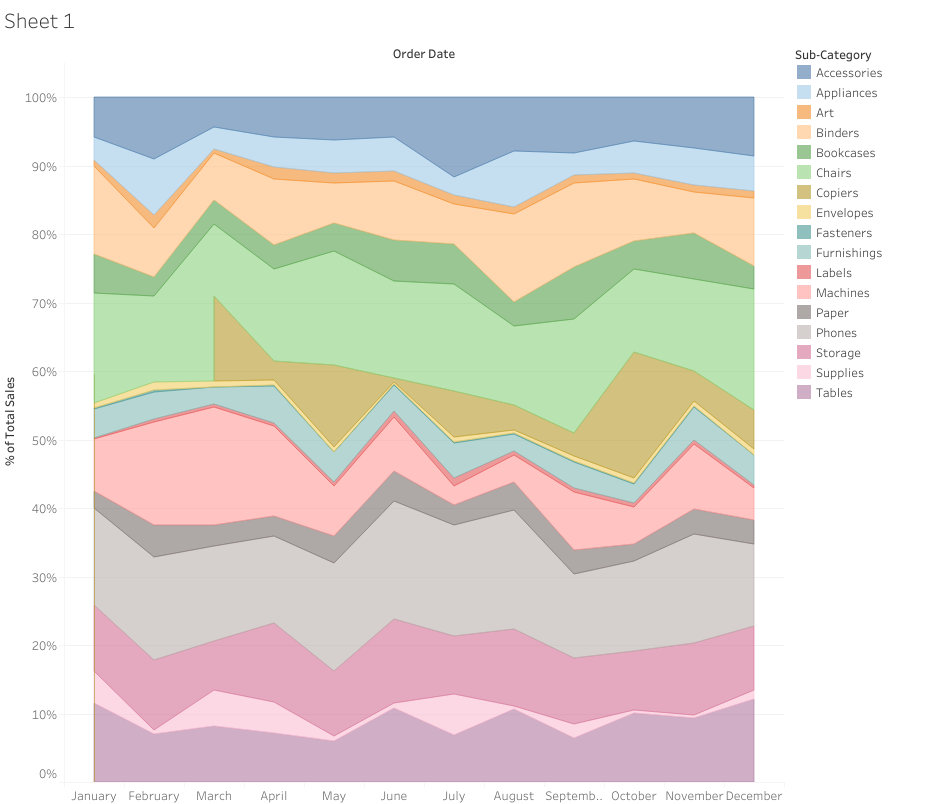
\includegraphics[height=1.8in]{Images/PT_C27_082322.png}
  \caption{Figure {\color{franklinblue} 1}: Percent of Corporate \\ Sales by Sub-Category}
\end{figure}
\end{textblock*}

\begin{textblock*}{5cm}(7.0cm,1.5cm)
\begin{figure}[htbp]
  \captionsetup{justification=centering}
  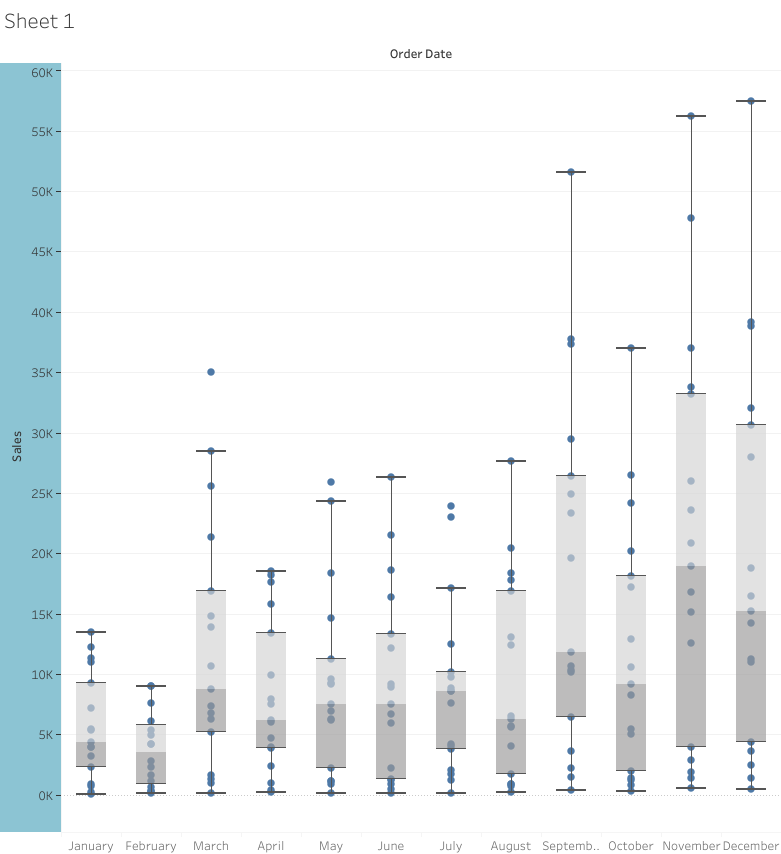
\includegraphics[height=1.8in]{Images/PT_C29_082522.png}
  \caption{Figure {\color{franklinblue} 2}: Box-and-Whiskers Plot \\ of Monthly Sub-Category Sales }
\end{figure}
\end{textblock*}

\end{frame}

\section{A Marketing Metric Example}

\begin{frame}[t]{An Advertising Campaign}
Suppose \href{https://www.abbottnutrition.com/}{Abbott Nutrition}, based in Columbus, Ohio, ran an advertising (ad) campaign announcing a new product line extension for a particular brand.  An \empr{ad campaign} is a collection of related ads that have a common theme (i.e., ``creatives'') and message.  The period during which the ads ran is frequently referred to as the \empr{campaign window}. \\
\vspace{1.5ex}
A campaign objective was to increase awareness of a new product line extension.  Specifically, the brand wanted to \empr{reach} about 50\% of its targeted audience with an \empr{average frequency} of 3.\footnote{Campaign reach is the number of different individuals exposed to a campaign within a given period of time. Campaign average frequency is the mean number of times that an individual is exposed to at least one campaign advertisement, given that he or she is indeed exposed to at least one campaign ad within a given period of time. %Thus \empr{frequency} is measured only among people who have been exposed to campaign under study.  
An introduction to traditional media planning is \cite{surmanek1996}.}  
\end{frame}

\begin{frame}[t]{Audience Selection via a Digital Platform}
Multiple media were used to execute the campaign, including a particular digital platform, \href{https://www.facebook.com/facebook/info/}{Facebook}.  \\
\vspace{1.5ex}
\href{https://www.facebook.com/Meta/}{Meta}, the company that owns Facebook, has many \underline{user-level} attributes, such as gender, age, location, \ldots, browsers, operating systems, \ldots, written content created by the user, content provided by the user via camera feature,  content a user viewed,  \ldots  \\
\vspace{1.5ex}
Facebook's ability to track users via a ``single-user login'' across devices and sessions represents a significant measurement advantage over more common cookie-based approaches. \\
\vspace{1.5ex}
The Meta attributes are used to select an \empr{audience}, which is a set of users who may be exposed to a focal campaign's ads.  A user's exposure is a function of the user logging into the platform, the platform's targeting algorithms, and the ad bidding process.   \\
\end{frame}

\begin{frame}[t]{A Campaign Contingency Table}
A deliverable provided by the platform after the campaign has been completed is Table \ref{tab:adcampct}, a $3 \times 2$ contingency table.   \\
\vspace{2.5ex}
% Table generated by Excel2LaTeX from sheet 'gender_exp_cont_table'
\begin{table}[htbp]
  \centering
  \captionsetup{justification=centering}
    \begin{tabular}{|l|r|r|r}
\cmidrule{2-4}    \multicolumn{1}{r|}{} & \multicolumn{1}{c|}{\cellcolor[rgb]{ .851,  .882,  .949}\textbf{Exposed}} & \multicolumn{1}{c|}{\cellcolor[rgb]{ .851,  .882,  .949}\textbf{Unexposed}} & \multicolumn{1}{c|}{\cellcolor[rgb]{ .851,  .882,  .949}\textbf{Total}} \\
    \midrule
    \rowcolor[rgb]{ .851,  .882,  .949} \textbf{Female} & \cellcolor[rgb]{ 1,  1,  1}8,777,045 & \cellcolor[rgb]{ 1,  1,  1}33,875,146 & \multicolumn{1}{r|}{\cellcolor[rgb]{ 1,  1,  1}42,652,191} \\
    \rowcolor[rgb]{ .851,  .882,  .949} \textbf{Male} & \cellcolor[rgb]{ 1,  1,  1}1,643,868 & \cellcolor[rgb]{ 1,  1,  1}6,722,339 & \multicolumn{1}{r|}{\cellcolor[rgb]{ 1,  1,  1}8,366,207} \\
    \rowcolor[rgb]{ .851,  .882,  .949} \textbf{Unknown} & \cellcolor[rgb]{ 1,  1,  1}19,869 & \cellcolor[rgb]{ 1,  1,  1}81,219 & \multicolumn{1}{r|}{\cellcolor[rgb]{ 1,  1,  1}101,088} \\
    \midrule
    \rowcolor[rgb]{ .851,  .882,  .949} \textbf{Total} & \cellcolor[rgb]{ 1,  1,  1}10,440,782 & \cellcolor[rgb]{ 1,  1,  1}40,678,704 & \cellcolor[rgb]{ 1,  1,  1} \\
\cmidrule{1-3}    \end{tabular}%
  \caption{Digital Platform Campaign Exposure Contingency Table}
  \label{tab:adcampct}%
\end{table}%
\vspace{-2.0ex}
While Table \ref{tab:adcampct} provides counts of users reached on Facebook, it does not provide cross-media reach nor frequency.  A single-source panel that sufficiently represents the population of interest may be used to estimate campaign cross-media reach and frequency. 
\end{frame}

\begin{frame}[t]{Another Campaign Objective }
The audience chosen for the Abbott Nutrition campaign, summarized in part by Table  \ref{tab:adcampct}, must have had a frequent shopper card (e.g., \href{https://www.gianteagle.com/save/giant-eagle-advantage-card}{Giant Eagle Advantage Card}, \href{https://www.kroger.com/pr/free-membership}{Kroger Plus Card}, \href{https://www.walgreens.com/topic/promotion/mywalgreens.jsp}{Walgreens myWalgreens Card}, \ldots) and must have had at least \$75 in monthly total frequent shopper card (FSC) gross sales for 10 of the 12 months before the campaign commenced.\footnote{The FSC historical purchase requirement is referred to as a \empr{static}.  This static ensures that an user is using his/her card with some regularity across time.} \\
\vspace{1.5ex}
By using the FSC requirement, we may link purchases to exposures to determine ad effectiveness. \\
\vspace{1.5ex}
The campaign ran for 4 weeks, where another of the campaign's objectives was to increase the conversion rate of brand purchase.  \\
\end{frame}

\begin{frame}[t]{Campaign Outcome Contingency Table}
Table \ref{tab:adcampoutct} is the outcome contingency table deliverable. For an exposed user to have a recorded purchase, the purchase must have occurred after the first ad exposure.  Purchase may have occurred during the 4-week campaign period or the 2 weeks thereafter. \\
\vspace{1.5ex}
% Table generated by Excel2LaTeX from sheet 'purchase_exp_cont_table'
\begin{table}[htbp]
  \centering
  \captionsetup{justification=centering}
    \begin{tabular}{|l|r|r|r}
\cmidrule{2-4}    \multicolumn{1}{r|}{} & \multicolumn{1}{c|}{\cellcolor[rgb]{ .851,  .882,  .949}\textbf{Exposed}} & \multicolumn{1}{c|}{\cellcolor[rgb]{ .851,  .882,  .949}\textbf{Unexposed}} & \multicolumn{1}{c|}{\cellcolor[rgb]{ .851,  .882,  .949}\textbf{Total}} \\
    \midrule
    \rowcolor[rgb]{ .851,  .882,  .949} \textbf{No Purchase} & \cellcolor[rgb]{ 1,  1,  1}10,208,648 & \cellcolor[rgb]{ 1,  1,  1}39,935,596 & \multicolumn{1}{r|}{\cellcolor[rgb]{ 1,  1,  1}50,144,244} \\
    \rowcolor[rgb]{ .851,  .882,  .949} \textbf{Purchase 1 Unit} & \cellcolor[rgb]{ 1,  1,  1}170,277 & \cellcolor[rgb]{ 1,  1,  1}547,698 & \multicolumn{1}{r|}{\cellcolor[rgb]{ 1,  1,  1}717,975} \\
    \rowcolor[rgb]{ .851,  .882,  .949} \textbf{Purchase 2 Units} & \cellcolor[rgb]{ 1,  1,  1}44,949 & \cellcolor[rgb]{ 1,  1,  1}149,006 & \multicolumn{1}{r|}{\cellcolor[rgb]{ 1,  1,  1}193,955} \\
    \rowcolor[rgb]{ .851,  .882,  .949} \textbf{Purchase 3+ Units} & \cellcolor[rgb]{ 1,  1,  1}16,908 & \cellcolor[rgb]{ 1,  1,  1}46,404 & \multicolumn{1}{r|}{\cellcolor[rgb]{ 1,  1,  1}63,312} \\
    \midrule
    \rowcolor[rgb]{ .851,  .882,  .949} \textbf{Total} & \cellcolor[rgb]{ 1,  1,  1}10,440,782 & \cellcolor[rgb]{ 1,  1,  1}40,678,704 & \cellcolor[rgb]{ 1,  1,  1} \\
\cmidrule{1-3}    \end{tabular}%
  \caption{Digital Platform Campaign Outcome Contingency Table}
  \label{tab:adcampoutct}%
\end{table}%
\end{frame}

\begin{frame}[t]{Campaign ROMI for the Facebook Execution}
For determining the campaign's ROMI, as executed on Facebook, we need:\\
\vspace{1.5ex}
\begin{enumerate}
 \item To know how the audience was selected.  
 \begin{itemize}
  \item More specifically, we need to know if ads delivered were via a design of experiment that used random selection of audience users to serve campaign ads. 
  \item If audience users were not randomly selected to serve an ad, then we have an \empr{observational data study}.\footnote{For a generalized introduction to causal inference for observational data studies using statistical and econometric techniques see \cite{imbens2015}. For an introduction to causal inference from a Bayesian Network perspective see \cite{pearl2018}.}
 \end{itemize}
 \vspace{0.0ex}
 Data resulting from a randomized experimental design will use different analytics than that of an observational data study.
\end{enumerate}
\end{frame}

\begin{frame}[t]{Weighting, Margins, and Ad Cost}
\begin{enumerate}
\setcounter{enumi}{1}
 \item Weights that project audience member sales metrics to all sales channels and purchase occasions. For example, we do not have product line purchase occasions outside of FSC retailers, such as Amazon, Walmart, Dollar General \ldots, and FSC purchase occasions where the card was not scanned.\footnote{For and introduction to the importance of proper weighting in statistics and econometrics see \cite{solon2015}.}
 \item Weighted average product line \$ sales and margin \$ sales per purchase occasion. 
 \item Campaign ad cost.  
\end{enumerate}
In summary, it can be challenging to provide sufficiently accurate and precise estimates of marketing metrics. 
\end{frame}

\section{Marketing Analytics Strategy and Metrics}

\begin{frame}[t]{Measuring Campaign Success}
Success of campaigns need to be measured.
\begin{itemize}
\item How much money to spend on them.
\item How to improve outcomes.
\end{itemize}
Marketing analytics is a continuous function of measuring results of campaigns.
\\
\vspace{1.5ex}
Campaign strategy steps are:
\\
\vspace{1.5ex}
\begin{figure}[htbp]
    \centering
    \captionsetup{justification=centering}
    
\includegraphics[clip, trim=0.0cm 0.0cm 0.0cm 0.0cm, width=1\textwidth]{Images/Picture1.png}  
    \caption{Figure {\color{franklinblue} 3}:  Campaign Strategy Steps}
    \label{fig:campstrag}
\end{figure} 
\end{frame}

\begin{frame}[t]{Campaign Strategy Steps are Cyclical in Nature}
\begin{figure}[htbp]
    \centering
    \captionsetup{justification=centering}
    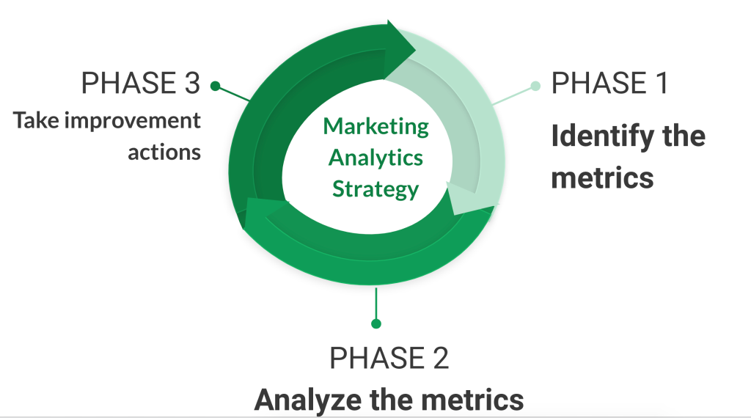
\includegraphics[clip, trim=0.0cm 0.0cm 0.0cm 0.0cm, width=1\textwidth]{Images/Picture2.png}  
    \caption{Figure {\color{franklinblue} 4}:  Cyclical Structure of Campaign Strategy Steps}
    \label{fig:campstrag}
\end{figure} 
\end{frame}

\begin{frame}[t]{Identify the Metrics}
Have a goal in mind. \\
\vspace{1.5ex} 
Determine the questions your data can address, and questions for which additional data will be needed. \\
\vspace{1.5ex}  
Metrics help bring meaning to the data. \\
\vspace{1.5ex}
\empr{Metrics} are quantifiable measures used to track the status of a marketing process.\\
\vspace{1.5ex}
Metrics help determine if goals are being achieved.
\end{frame}

\begin{frame}[t]{Analyze the Metrics}
Companies must implement systems to track the important metrics.\\
\vspace{1.5ex}
\begin{itemize}
\item Web Analytics
\item Marketing Dashboards\footnote{Best-in-class solutions are fully automated, scalable, and updated on a periodic cadence that meets the needs of the business.}
\end{itemize}
Compare current state to benchmarks. \\
\vspace{1.5ex}
\begin{itemize}
\item Historical Trends
\item Industry Average Performance
\end{itemize}
The most important step is to determine the root cause of why metrics perform the way they do.
\end{frame}

\begin{frame}[t]{Curata's Content Metrics and Model Structure}
\begin{figure}[htbp]
    \centering
    \captionsetup{justification=centering}
    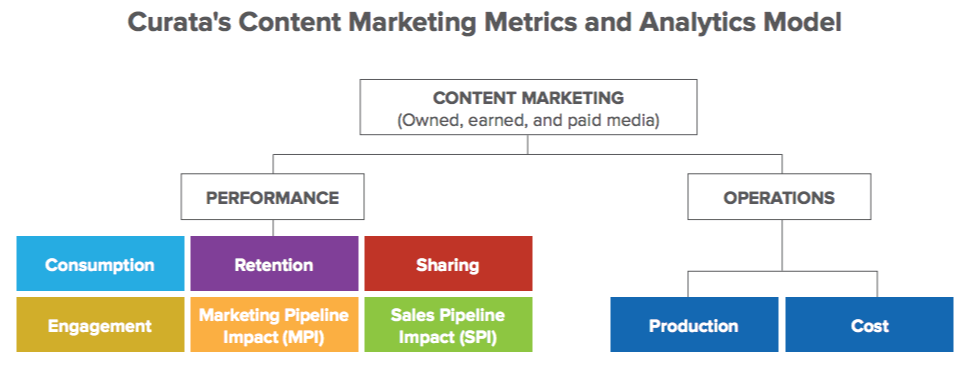
\includegraphics[clip, trim=0.0cm 0.0cm 0.0cm 0.0cm, width=1\textwidth]{Images/Figure_12_2.png}  
    \caption{Figure {\color{franklinblue} 5}:  Curata's Metrics and Model Structure}
    \label{fig:curata}
\end{figure} 
\end{frame}

\begin{frame}[t]{Curata's Content Metrics and Analytics Model}
\begin{figure}[htbp]
    \centering
    \captionsetup{justification=centering}
    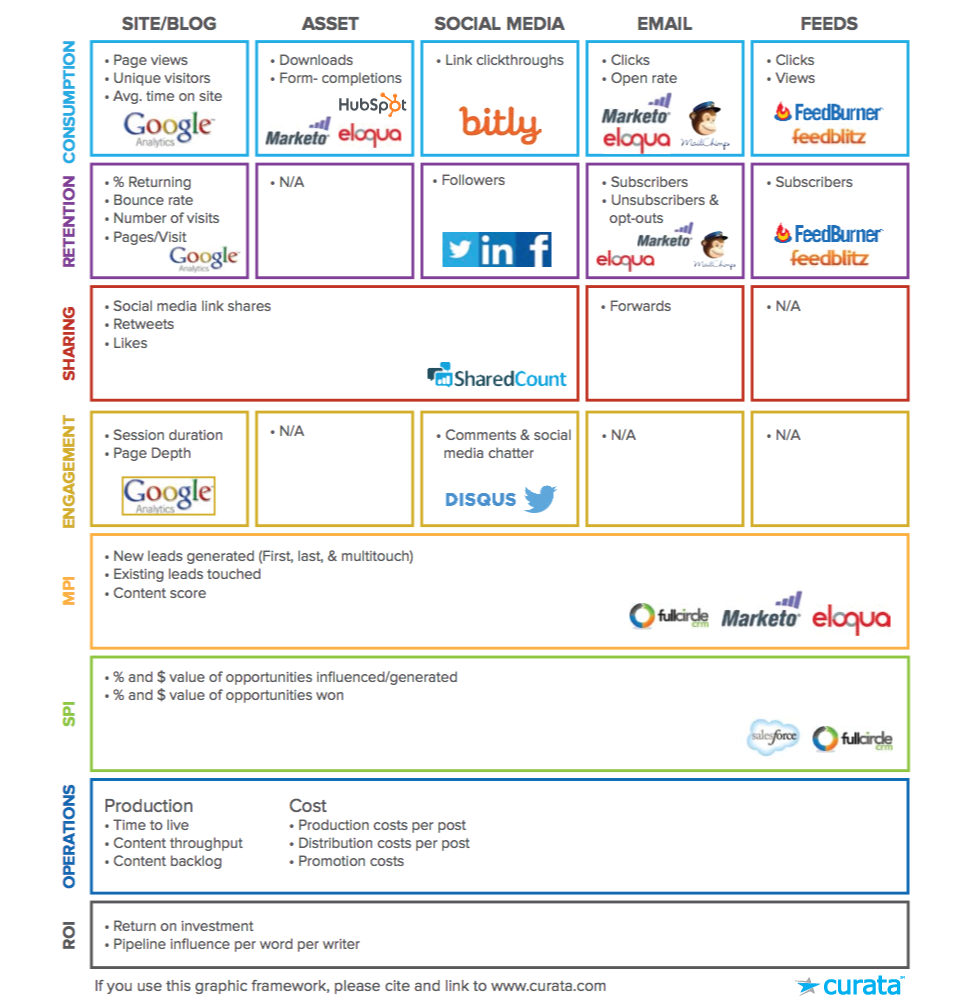
\includegraphics[clip, trim=0.0cm 0.0cm 0.0cm 0.0cm, width=0.60\textwidth]{Images/Figure_12_3.png}  
    \caption{Figure {\color{franklinblue} 6}:  Curata's Content Marketing Metrics and Analytics Model}
    \label{fig:curata}
\end{figure} 
\end{frame}

\begin{frame}[t]{Google's Universal Analytics}
\href{https://analytics.google.com/analytics/academy/}{Google's Universal Analytics} permitted one to measure advertising performance, as well as track Flash, video, and social networking sites and applications.  It has been sunsetted.\\
\vspace{1.5ex}
\begin{figure}[htbp]
    \centering
    \captionsetup{justification=centering}
    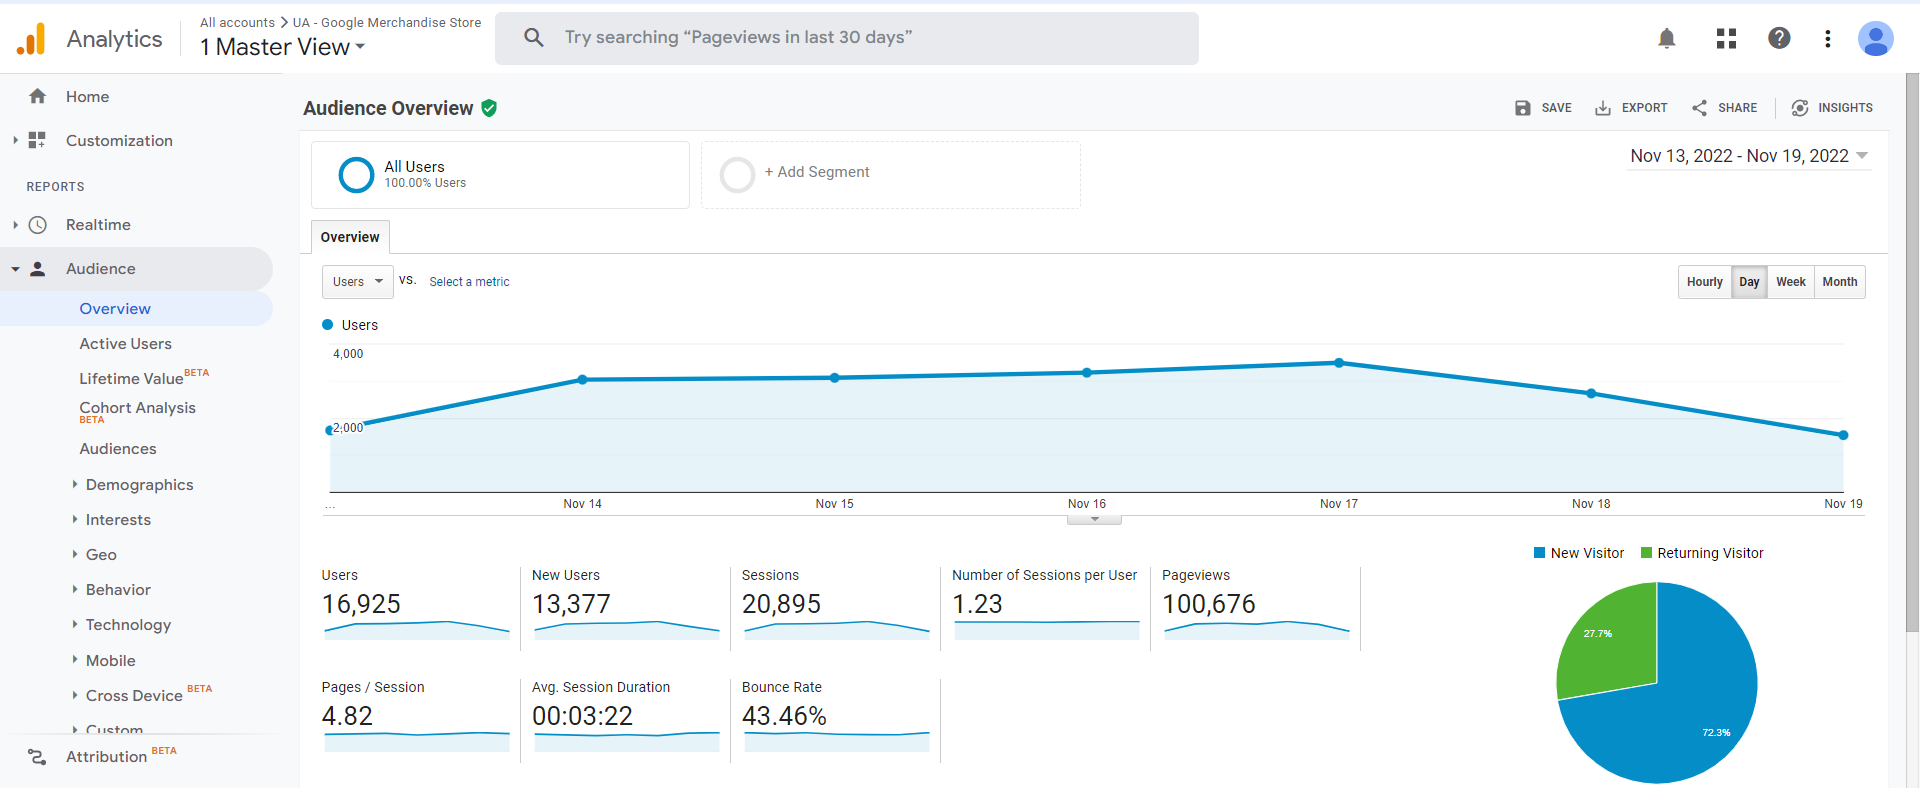
\includegraphics[clip, trim=0.0cm 0.0cm 0.0cm 0.0cm, width=1\textwidth]{Images/Google_Analytics.png}  
    \caption{Figure {\color{franklinblue} 7}:  Google Analytics Interface}
    \label{fig:googleanalytics}
\end{figure} 

\end{frame}

\begin{frame}[t]{Google Analytics 4}
\href{https://support.google.com/analytics/answer/10089681?hl=en}{Google Analytics 4} is a new kind of property designed for the future of digital measurement.  It replaced Universal Analytics. \\
\vspace{1.5ex}
\begin{itemize}
\item Collects both website and application data to better understand the customer journey.
\item Uses event-based data instead of session-based data.
\item Includes privacy controls such as cookie-less measurement, and behavioral and conversion modeling.\footnote{The Appendix provides an overview of the (historical) use of cookies for providing limited persistent user privacy choices and tracking in the evolving multi-device, multi-environment
digital landscape or ``state management''.}
\item Predictive capabilities offer guidance without complex models.
\item Direct integrations to media platforms help drive actions on the measured website or application.
\end{itemize}
\end{frame}

\begin{frame}[t]{Nielsen Ad Intelligence}
\href{https://www.nielsen.com/solutions/media-planning/ad-intelligence/?gclid=Cj0KCQiA4OybBhCzARIsAIcfn9mptPSPlhWwtKcR07kqOhwDHAjAxI0tc_CecLGS0xyp-ag17ENm02caAvAJEALw_wcB&gclsrc=aw.ds}{Nielsen Ad Intel} is the most comprehensive source of local, national and international advertising spend data available today. \\
\vspace{-2.0ex}
\begin{figure}[htbp]
    \centering
    \captionsetup{justification=centering}
    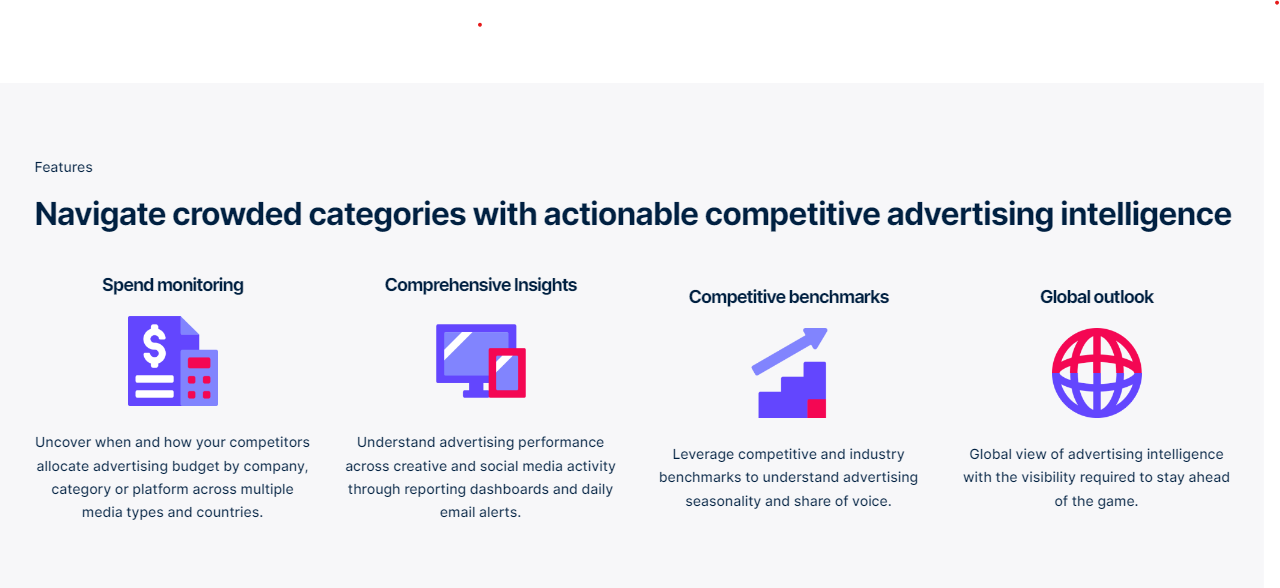
\includegraphics[clip, trim=0.0cm 0.0cm 0.0cm 0.0cm, width=1\textwidth]{Images/Nielsen_Ad_Intel.png}  
    \caption{Figure {\color{franklinblue} 8}:  Nielsen Ad Intelligence Benefits}
    \label{fig:nielsenadintel}
\end{figure} 
\end{frame}

\begin{frame}[t]{IRI, Spins and NielsenIQ Syndicated Data}
\empr{Syndicated data} refers to an aggregated collection of retail sales market data. Unlike direct point-of-sale retail data, syndicated data grants an industry, market, or categorical look at the data rather than just featuring an individual retailer, brand, or product. \\
\small
\begin{itemize}
\item The organizations that collect, curate and sell consumer packaged goods (CPG) market data -- NielsenIQ, IRI and Spins offer increasingly distinct syndicated data.  This data is primarily used by CPG manufacturers (e.g., Coca-Cola, P\&G, Kraft-Heinz, \dots), and retailers (e.g., Walmart, Target, Sam's Club, CVS, Kroger, Dollar General, \ldots) who share data with the syndicated data providers. \\
\item 
The Retail Tracking Service of  \href{https://www.npd.com/products/retail-tracking/}{NPD}
sources point-of-sale data from over 600,000 retail locations, plus e-commerce and mobile platforms. This data is primarily used by retailers selling products other than those of CPG manufacturers.
\end{itemize} 
\end{frame}

\begin{frame}[t]{Take Improvement Actions}
Taking actions that improve marketing is the most difficult step in the process. \\
\vspace{1.5ex}
Since changes are not always obvious, marketers use analytical and creative skills to develop solutions. For example, A/B testing allows marketers to make isolated changes until the best performing marketing effort can be achieved. \\
\vspace{1.5ex}
Firms need to invest their resources in areas that need the most improvement, or reallocate resources to more productive and efficient marketing tactics.
\end{frame}

\begin{frame}[t]{Managing Analytics During the Campaign Life Cycle}
\begin{figure}[htbp]
    \centering
    \captionsetup{justification=centering}
    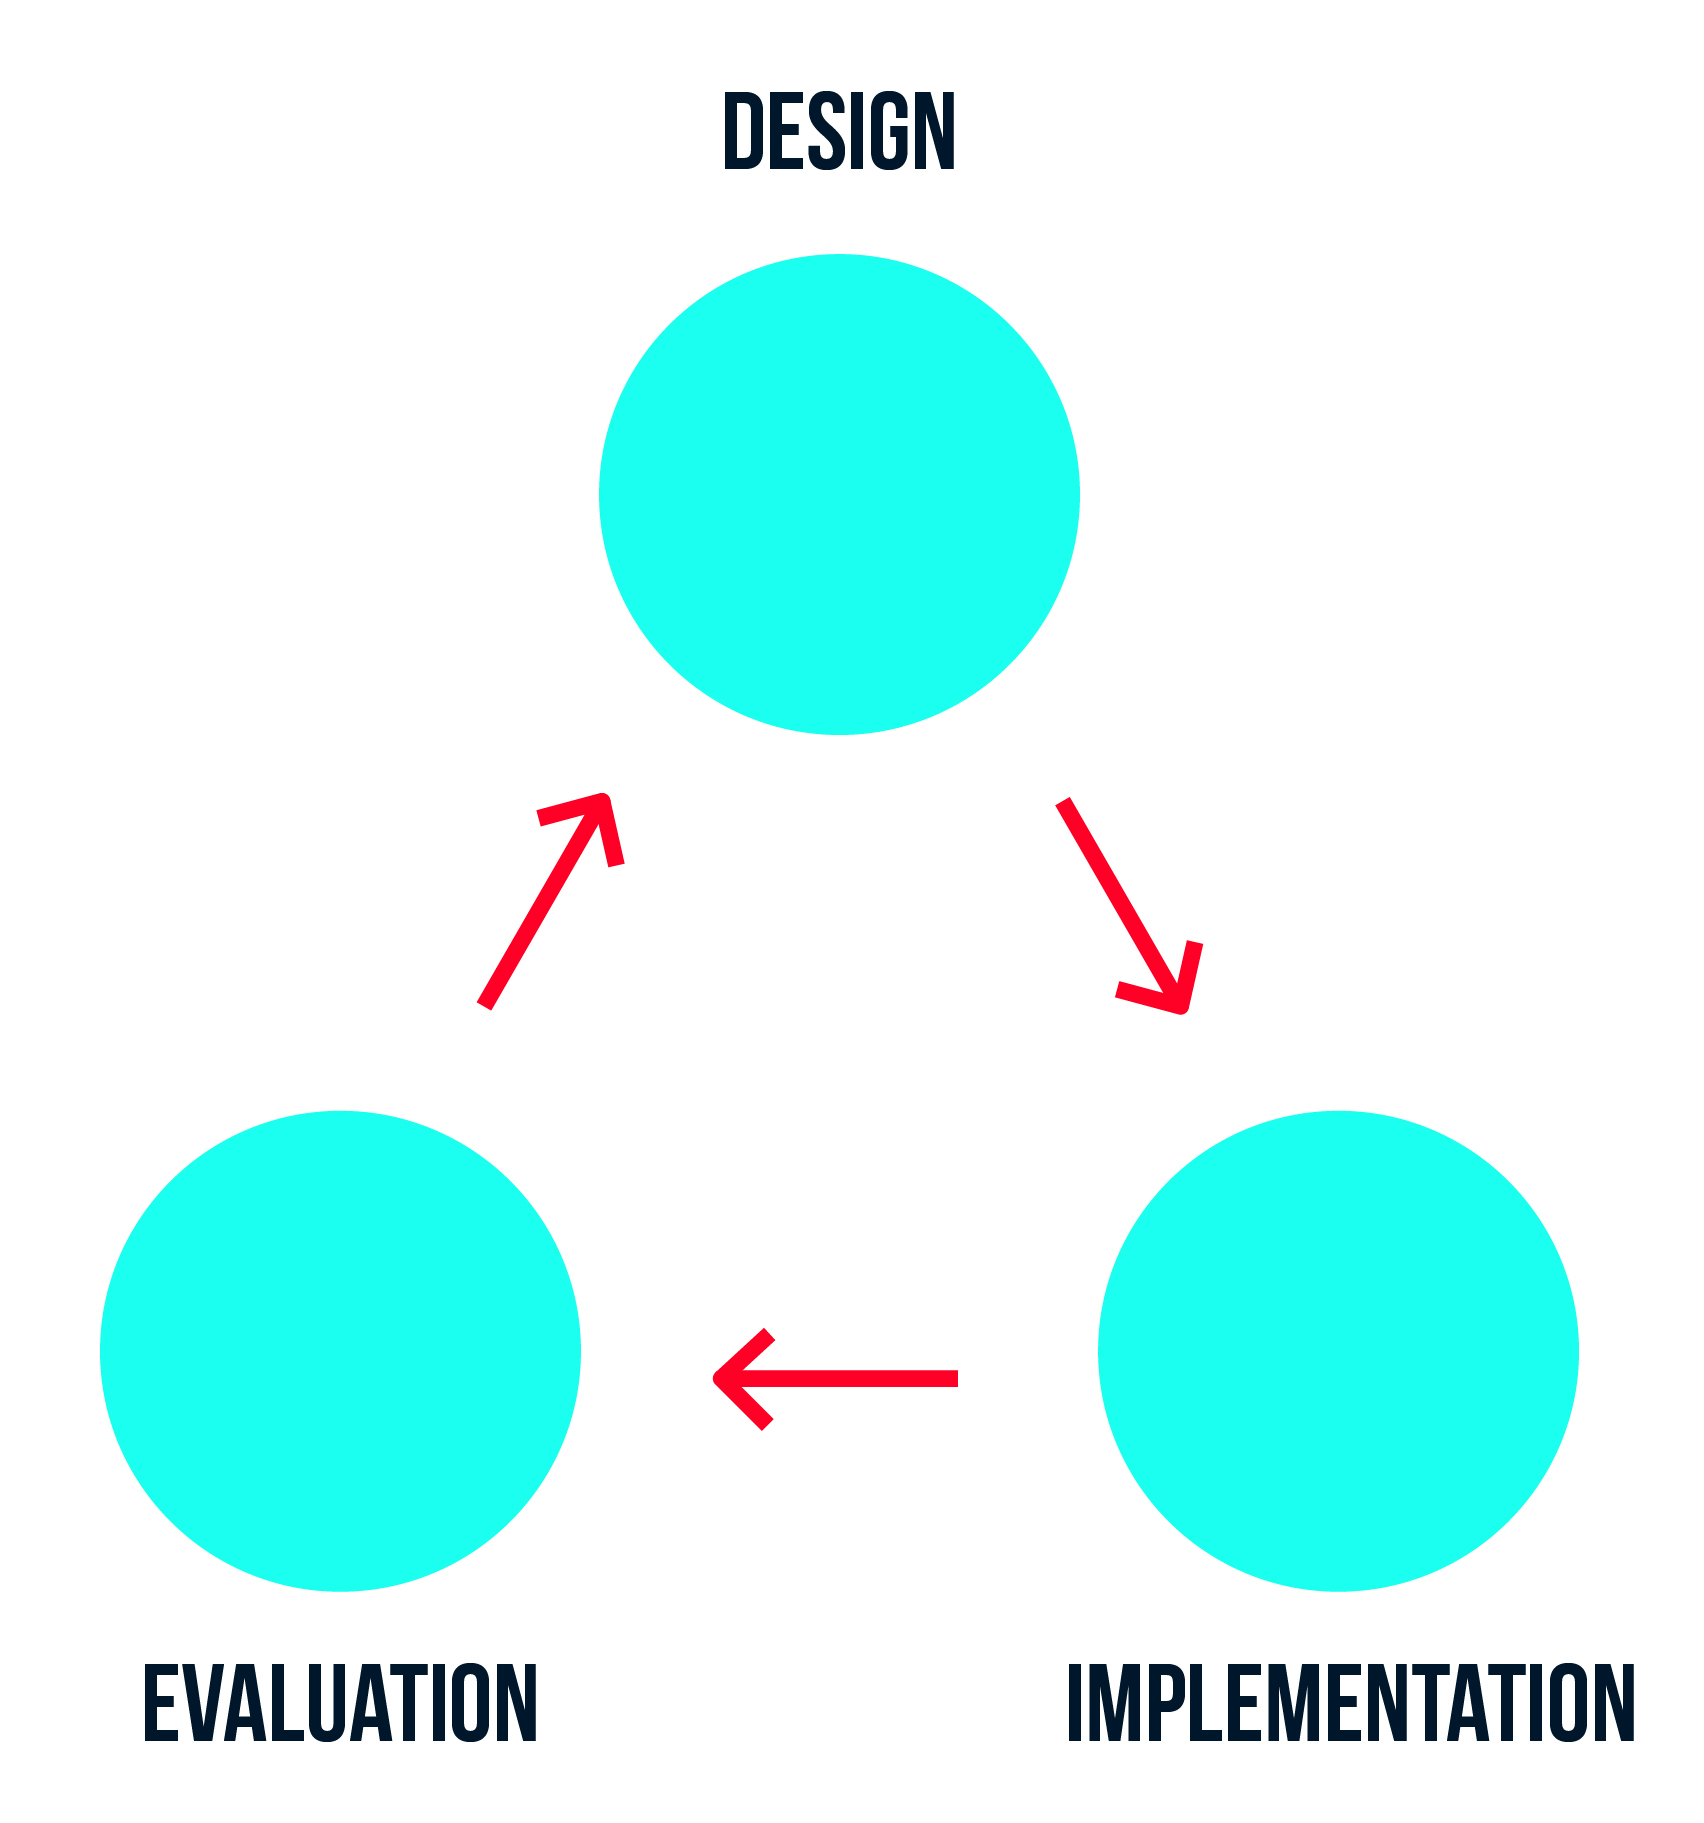
\includegraphics[clip, trim=0.0cm 0.0cm 0.0cm 0.0cm, width=0.6\textwidth]{Images/Figure_12_4_2.jpg}  
    \caption{Figure {\color{franklinblue} 9}: Managing Analytics During the Campaign Life Cycle}
    \label{fig:camplc}
\end{figure} 
\end{frame}

\begin{frame}[t]{Design}
The first stage is the \underline{design} of a marketing campaign. This often starts with exploratory research, for which analytics can be helpful. \\
\vspace{1.5ex}
\begin{itemize}
\item Web behavior flow, such as visit counts, patterns, and clicks.
\item Social media analytics, such as likes, follows and mentions. 
\item Sentiment analysis, which is a natural language processing (NLP) technique used to determine whether data is positive, negative or neutral. 
\item Reviewing brand trackers, such as the brand equity tracker available from \href{https://theharrispoll.com/solutions/harris-brand-platform/brand-equity/}{Harris}.
\item Conducting limited scale A/B tests. 
\end{itemize}
\end{frame}


\begin{frame}[t]{Implementation}
Flawless implementation of the design puts the campaign in a position to succeed. \\
\vspace{1.5ex}
It is vitally important to carefully and regularly monitor results and making adjustments when necessary.  \\
\vspace{1.5ex}
For digital campaigns, use real-time analytics to ensure tags are correctly firing and the proper data is being collected.
\end{frame}

\begin{frame}[t]{Evaluation}
Marketing campaigns generally have a specific set of goals, such as:
\vspace{-0.5ex}
\small
\begin{itemize} 
\item Targeted number of conversions.
\item Impressions served and viewed.
\item Number of web site interactions.
\item Number of web site page views.
\item \ldots 
\end{itemize}
\vspace{-0.5ex}
Campaign goals are measurable and can be tracked with analytics. \\
\vspace{1.5ex}
Evaluate whether a campaign has met its goals or not. \\
\vspace{1.5ex} 
Determine how many resources should be spent in the future, if any.
\end{frame}

\section{Strategic Marketing Analytics}

\begin{frame}[t]{There are a Wide Range of Metrics}
The range of metrics that companies can employ vary from those that are mandatory for contractual purposes (i.e., a consulting firm that only gets paid if it can show results) to those that voluntarily track metrics for increased efficiency, reductions in complaints, and greater profits. \\
\vspace{1.5ex}
Overall, \empr{strategic metrics}, also known as \empr{support metrics}, should reflect and support the various strategies for all aspects of the firm along with customer expectations.\\
\vspace{1.5ex}
\begin{figure}[htbp]
    \centering
    \captionsetup{justification=centering}
    
\includegraphics[clip, trim=0.0cm 0.0cm 0.0cm 0.0cm, width=1\textwidth]{Images/Picture3.png}  
    \caption{Figure {\color{franklinblue} 10}:  Classification of Strategic Metrics}
    \label{fig:campstrag}
\end{figure} 
\end{frame}

\begin{frame}[t]{Brand Metrics}
\empr{Brand metrics} shed light on customers' understanding of, and relationship with, the brand.  These metrics are a composite of individual customer responses.  \\
\vspace{1.5ex}
\footnotesize
\begin{table}[htbp]
  \centering
  \captionsetup{justification=centering}
    \begin{tabular}{|c|l|l|}
    \toprule
   % \rowcolor[rgb]{ .851,  .882,  .949} \textbf{Sample} & \textbf{Sample Mean} & \textbf{Sample} & \textbf{Sample Mean} & \textbf{Sample} & \textbf{Sample Mean}  \\
   %\midrule
    Metric & Definition & Vendors\\
    \midrule
    \multirow{2}{*}{Brand Recall} & The ability to retrieve the brand & \multirow{8}{1.6cm}{\href{https://www.comscore.com/Products/Marketing-Impact/Brand-Effectiveness}{Comscore}, \href{https://www.ipsos.com/en-us/brand-equity-measurement}{Ipsos}, \href{https://www.kantar.com/expertise/brand-growth/brand-tracking}{Kantar}, \href{https://marketcast.com/}{MarketCast}, \href{https://www.nielsen.com/solutions/marketing-optimization/brand-impact/}{Nielsen}}  \\
    & from memory. & \\
    \cmidrule{1-2}
    \multirow{2}{*}{Brand Recognition} & The ability of the customer to &  \\ 
    & confirm a prior exposure to a brand. & \\
    \cmidrule{1-2}
    \multirow{2}{*}{Brand Depth} & The ease with which a brand & \\
    & comes to mind. & \\
    \cmidrule{1-2}
    \multirow{2}{*}{Brand Breadth} & The range of usage scenarios for  &  \\
    & a brand. & \\
  \bottomrule
     \end{tabular}%
  \caption{Brand Metrics}
  \label{tab:mrandmetrics}%
\end{table}%
\end{frame}

\begin{frame}[t]{Customer Metrics}
\empr{Customer metrics} measure the performance of individual customer relationships.\\
\vspace{1.5ex}
\footnotesize
\begin{table}[htbp]
  \centering
  \captionsetup{justification=centering}
    \begin{tabular}{|c|l|}
    \toprule
   % \rowcolor[rgb]{ .851,  .882,  .949} \textbf{Sample} & \textbf{Sample Mean} & \textbf{Sample} & \textbf{Sample Mean} & \textbf{Sample} & \textbf{Sample Mean}  \\
   %\midrule
    Metric & Definition \\
    \midrule
   Customer Lifetime Value  & The present value of the future cash flows \\
    (LTV)  & attributed to the customer relationship.\footnote{A more precise definition of LTV is the net present value of profits linked to a specific customer once the customer has been acquired, after subtracting incremental costs associated with marketing, selling, production and servicing over the customer's lifetime. Given this definition one needs to, (1) forecast future sales of a customer, (2) compute incremental costs per customer, and (3) determine the relevant discount rate to use in the present value calculation.}\\  
    \midrule
   \multirow{3}{*}{Margin} & The revenue generated by customers less the \\
           & variable cost it takes to deliver the good or \\
           & service to the customer.%\footnote{This is a component of the P\&L statement.}
            \\ 
    \midrule
   \multirow{2}{*}{Retention Rate} & The percentage of customers who remain loyal \\
    & over time.\\
    \bottomrule
     \end{tabular}%
  %\caption{Customer Metrics}
  \label{tab:custmetrics}%
\end{table}%
\end{frame}

\begin{frame}[t]{Customer Metrics - Profit and Satisfaction}
\footnotesize
\begin{table}[htbp]
  \centering
  \captionsetup{justification=centering}
    \begin{tabular}{|c|l|}
    \toprule
   % \rowcolor[rgb]{ .851,  .882,  .949} \textbf{Sample} & \textbf{Sample Mean} & \textbf{Sample} & \textbf{Sample Mean} & \textbf{Sample} & \textbf{Sample Mean}  \\
   %\midrule
    Metric & Definition \\
    \midrule
    \multirow{2}{*}{Customer Profit} & Defined as customer revenue minus customer  \\
                    & costs.\footnote{This term has more flexibility in its definition than Margin.} \\
    \midrule 
    \multirow{3}{*}{Customer Satisfaction} & Generally measured on a 1 to 5 scale, in which \\
                          & customers declare their satisfaction with the  \\ 
                          & brand in general or brand specific attributes. \\
    \midrule 
    \multirow{3}{*}{Discount Rate} & %The cost of capital for an organization.\footnote{It is similar to an interest rate on a loan.}
    The interest rate used to determine the present \\ 
                  & value of future cash flows in a discounted cash  \\
                  & flow analysis.\footnote{It is different than the \empr{cost of capital}, which refers to the required return necessary to make a project or investment worthwhile. This is specifically attributed to the type of funding used to pay for the investment or project. If it is financed internally, it refers to the cost of equity. If it is financed externally, it is used to refer to the cost of debt.} \\
    \bottomrule
     \end{tabular}%
  \caption{Customer Metrics}
  \label{tab:custmetrics}%
\end{table}%
\end{frame}
\begin{frame}[t]{A Simple Customer Lifetime Value Formula}
\begin{figure}[htbp]
    \centering
    \captionsetup{justification=centering}
    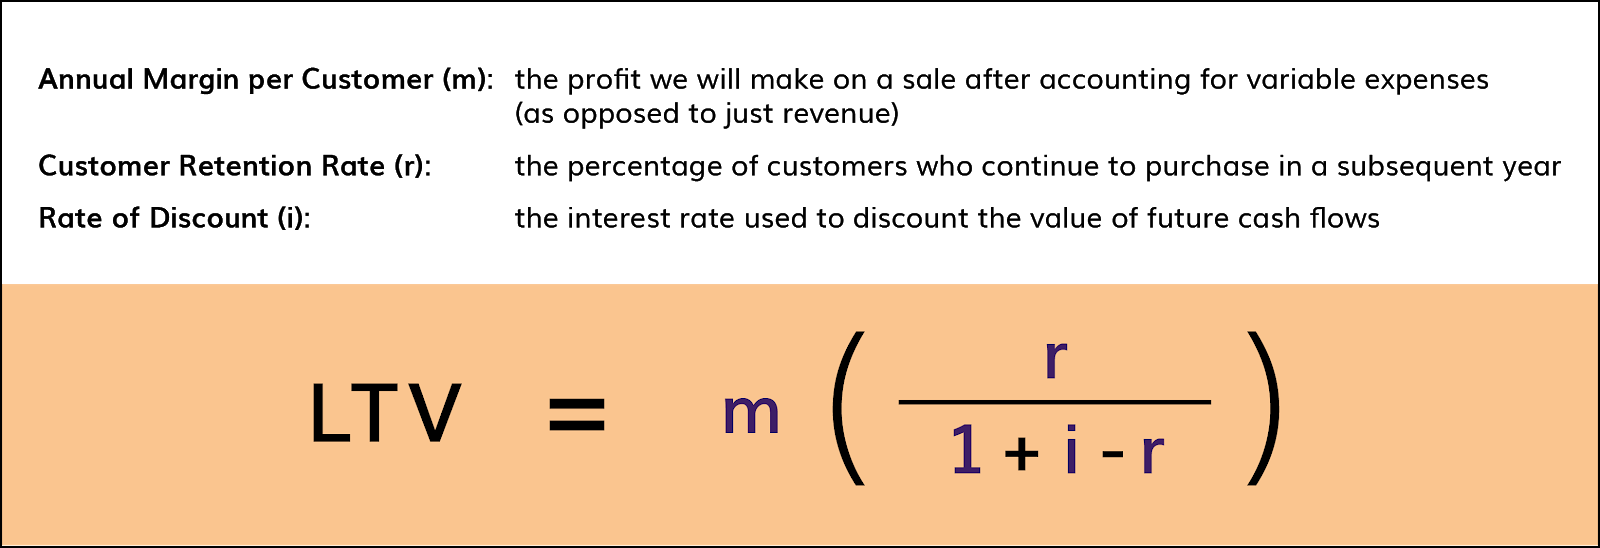
\includegraphics[clip, trim=0.0cm 0.0cm 0.0cm 0.0cm, width=1\textwidth]{Images/Figure_12_4.png}  
    \caption{Figure {\color{franklinblue} 11}: A Simple Customer Lifetime Value Formula}
    \label{fig:camplc}
\end{figure} 
\vspace{-2.0ex}
\small
LTV requires a projection of future cash flows from a customer relationship. Formulations of LTV differ with respect to the treatment of the initial margin and acquisition spending. Many times LTV is calculated by segment, such as by acquisition channel. \\
\vspace{1.5ex}
Customer relationship management decisions should be made with the objective of improving LTV. Acquisition budgets should be based on LTV.  
\end{frame}

\begin{frame}[t]{Digital Marketing Metrics}
\empr{Digital marketing metrics} measure the success of marketing efforts in digital media environments.\\
\vspace{0.0ex}
\footnotesize
\begin{table}[htbp]
  \centering
  \captionsetup{justification=centering}
    \begin{tabular}{|c|l|}
    \toprule
    Metric & Definition \\
    \midrule
    \multirow{3}{*}{Conversion} & Counted as the number of people who have taken a \\
                              & desired marketing outcome as defined by the marketing \\
                              & team.\footnote{Examples include completing a checkout on an e-commerce site, completing a lead  form, subscribing for a service, or signing up for a newsletter.} \\
   \midrule 
    \multirow{2}{*}{Impressions} & Counted as the number of times marketing content has\\
                                & been displayed to a person.\\
    \midrule
   Reach & The number of unique people who received impressions. \\
    \midrule 
   Conversion Rate & Total conversions divided total reach. \\ 
   \midrule 
    Micro Conversion & The conversion rate at the campaign or platform \\
    Rate & level. \\
    \bottomrule
     \end{tabular}%
  %\caption{Customer Metrics}
  \label{tab:custmetrics}%
\end{table}%
\end{frame}

\begin{frame}[t]{Digital Marketing Metrics Continued}
\footnotesize
\begin{table}[htbp]
  \centering
  \captionsetup{justification=centering}
    \begin{tabular}{|c|l|}
    \toprule
    Metric & Definition \\
    \midrule
   \midrule 
   Conversion & The portion of customers who make it through to the \\
   Funnel             & next level of each step in the journey from (first)  \\
    Rate                 & impression to conversion. \\ 
    \midrule
   Lead to  &  Total number of sales leads divided by the total number \\
   Close Ratio & of sales. \\
    \midrule 
    \multirow{2}{*}{Visits} & The total number of times that visitors come to a website \\ 
   & or webpage.\\ 
   \midrule
   Unique   & The total number of unique visitors to a website or \\
    Visitors                & webpage.\footnote{At times determined by IP address.}  \\
   \midrule 
  New Sessions & The total number of first time-site visitors.\footnote{Cookie deletion on a browser will create a new session upon visiting the website.} \\
  \midrule
  Site Time & The amount of time a customer spends on a website.\footnote{For Google Universal Analytics, Average (Session) Duration is reported.} \\
  \midrule
     \end{tabular}%
  %\caption{Customer Metrics}
  \label{tab:custmetrics}%
\end{table}%
\end{frame}

\begin{frame}[t]{Digital Marketing Metrics Continued}
\footnotesize
\begin{table}[htbp]
  \centering
  \captionsetup{justification=centering}
    \begin{tabular}{|c|l|}
    \toprule
    Metric & Definition \\
    \midrule
  Direct  & The number of people who typed in the URL, or used a \\
  Traffic &  bookmark, to get to a website.\\
  \midrule 
   \multirow{2}{*}{Referrals} & Total number of people who clicked a link from another \\
    & website to get to the website of interest.\\
   \midrule 
    \multirow{4}{*}{Organic Traffic} & Total number of people who reached the website by \\
                  & performing a search from sites like Google or Bing, and \\
                  & used an \underline{unpaid listing} on the search engine's results\\
                  & pages (SERPs). \\
    \midrule
    \multirow{2}{*}{Social Traffic} & The number of people who found the website via social \\
                  & media. \\
    \midrule 
    \multirow{2}{*}{Bounce Rate} & The percentage of people who leave a website after \\
              & viewing only one page. \\ 

    \bottomrule
     \end{tabular}%
  %\caption{Customer Metrics}
  \label{tab:custmetrics}%
\end{table}%
\end{frame}

\begin{frame}[t]{Digital Marketing Metrics Continued}
\footnotesize
\begin{table}[htbp]
  \centering
  \captionsetup{justification=centering}
    \begin{tabular}{|c|l|}
    \toprule
    Metric & Definition \\
    \midrule
    \midrule
     Click- & In Google Analytics 4, CTR is the  number of  clicks \\ 
     Through & that an ad receives divided by the number of times \\ 
    Rate (CTR) & the ad is shown: clicks ÷ impressions = CTR. \\
   \midrule 
   Customer & Determined by the total marketing costs over a period \\
    Acquisition & of time divided by the total amount of new customers \\
     Cost (CAC) & in that same time period.\\ 
    \midrule
   \multirow{3}{*}{Open Rate} &  The total number of people who open an email sent \\
   & to them divided by the total number of people to whom\\
   & the email was sent.\\
    \midrule 
   \multirow{2}{*}{Mobile Rate} & The number of people who see marketing content through \\
   & a mobile device. \\ 
    \bottomrule
     \end{tabular}%
  \caption{Digital Marketing Metrics}
  \label{tab:digitalmetrics}%
\end{table}%
\end{frame}

\begin{frame}[t]{Development Metrics}
\empr{Development process metrics}, or simply \empr{development metrics} measure a company's ability to leverage competitive advantage and product or service development. \\
\vspace{1.5ex}
It is recommended to divide each development project into the following kinds of metrics: low cost, customization, quality, responsiveness and innovation. \\
\vspace{1.5ex}
\footnotesize
\begin{table}[htbp]
  \centering
  \captionsetup{justification=centering}
    \begin{tabular}{|c|l|}
    \toprule
    Metric Type & Explanation \\
    \midrule
   Low Cost  &  Measures the ability to deliver goods and services at \\
   Metrics & sufficiently minimal cost.\\
   \midrule 
   Customization & Measures the ability to tailor products and services \\
   Metrics & to customers. \\
    \midrule
   \multirow{2}{*}{Quality Metrics} & Measures the ability to produce high-quality products \\
   & and services. \\
  \bottomrule
     \end{tabular}%
  %\caption{Development Metrics}
  \label{tab:custmetrics}%
\end{table}%
\end{frame}

\begin{frame}[t]{Development Metrics - Response and Innovation}
\footnotesize
\begin{table}[htbp]
  \centering
  \captionsetup{justification=centering}
    \begin{tabular}{|c|l|}
    \toprule
     Metric Type & Explanation \\
    \midrule
   Responsive & Measures whether companies are attentive to customer \\ 
   Metrics & needs. \\ 
      \midrule 
   Innovation & Measure a company's ability to invent new products \\
   Metrics & and services.  \\ 
    \bottomrule
     \end{tabular}%
  \caption{Development Metrics}
  \label{tab:custmetrics}%
\end{table}%
\vspace{-2.0ex}
\normalsize
A \empr{key performance indicator} (KPI) is a metric that is vitally important for the success of the firm. \\
\vspace{1.5ex}
The first task of every good marketing analytics professional should be to understand what is important to the firm, and identifying which metrics are KPIs.
\end{frame}

\section{Appendix}

\begin{frame}[t]{Defining the Cookie}
% https://mcgaw.io/blog/end-of-third-party-cookies-ios14-itp/#gs.4d0m2j
% https://www.iab.com/insights/glossary-of-terminology/#index-3
% https://blog.google/products/chrome/privacy-sandbox-tracking-protection/
% https://blog.sentry.io/we-removed-advertising-cookies-heres-what-happened/
% https://www.iab.com/wp-content/uploads/2015/08/IABDigitalSimplifiedMobileCookies.pdf
% https://www.iab.com/wp-content/uploads/2017/06/Mobile-Identity-Guide-for-Marketers-Report.pdf
% https://www.iab.com/wp-content/uploads/2023/09/IAB-MRC-Retail-Media-Measurement-Guidelines_For-Public-Comment-1.pdf
% https://www.devx.com/terms/html5-cookie/
% https://splitmetrics.com/glossary/what-is-idfa/#:~:text=How%20is%20IDFA%20changing%20in,apps%20and%20websites%20using%20IDFA.
% https://www.publift.com/blog/what-is-universal-id-and-how-can-it-help-publishers
% https://www.iab.com/wp-content/uploads/2015/08/IABDigitalSimplifiedMobileCookies.pdf
The \href{https://www.iab.com/}{Interactive Advertising Bureau} (IAB) is comprised of more than 700  media companies, brands, agencies, and technology firms that are responsible for selling, delivering, and optimizing digital ad marketing campaigns.  The trade group fields research on interactive advertising, while also educating brands, agencies, and the wider business community about digital marketing. \\
\vspace{1.5ex}
The \href{https://www.iab.com/insights/glossary-of-terminology/}{IAB glossary} defines \href{https://www.iab.com/insights/glossary-of-terminology/\#index-3}{\empr{cookie}}, also known as an \empr{HTTP cookie}, \empr{web cookie}, or \empr{browser cookie}, as a string of text sent from a web server to a user's browser that the browser is expected to send back to the web server in subsequent interactions.\\
\vspace{1.5ex}
\small
\begin{itemize}
\item A cookie has a few core attributes: the \empr{cookie value}, the \href{https://www.iab.com/insights/glossary-of-terminology/\#index-4}{\empr{domain (name)}} and \empr{path} within which it is valid, and the \empr{cookie expiry}. There are other attributes as well that limit the cookie to https-only transactions, or hide it from JavaScript. 
\end{itemize}
\end{frame}

\begin{frame}[t]{Persistent and Session Cookies}
\small
\begin{itemize}
  \item The domain and path define the scope of the cookie -- they tell the browser that cookies should only be sent back to the server for the given domain and path. \\
  \vspace{1.5ex}
  Cookies that do not have a specific expiration date and time are automatically deleted when the web browser is next closed. \\
  \vspace{1.5ex}
  Cookies with a set expiry time are considered \empr{persistent cookies}, while cookies without set expiry times are considered \empr{session cookies}.
\end{itemize}
\normalsize
Given recent data privacy changes in the industry, one frequently confronts \empr{cookie consent banners}. 
\end{frame}

\begin{frame}[t]{Cookie Consent Banner}
\begin{figure}[htbp]
    \centering
    \captionsetup{justification=centering}
    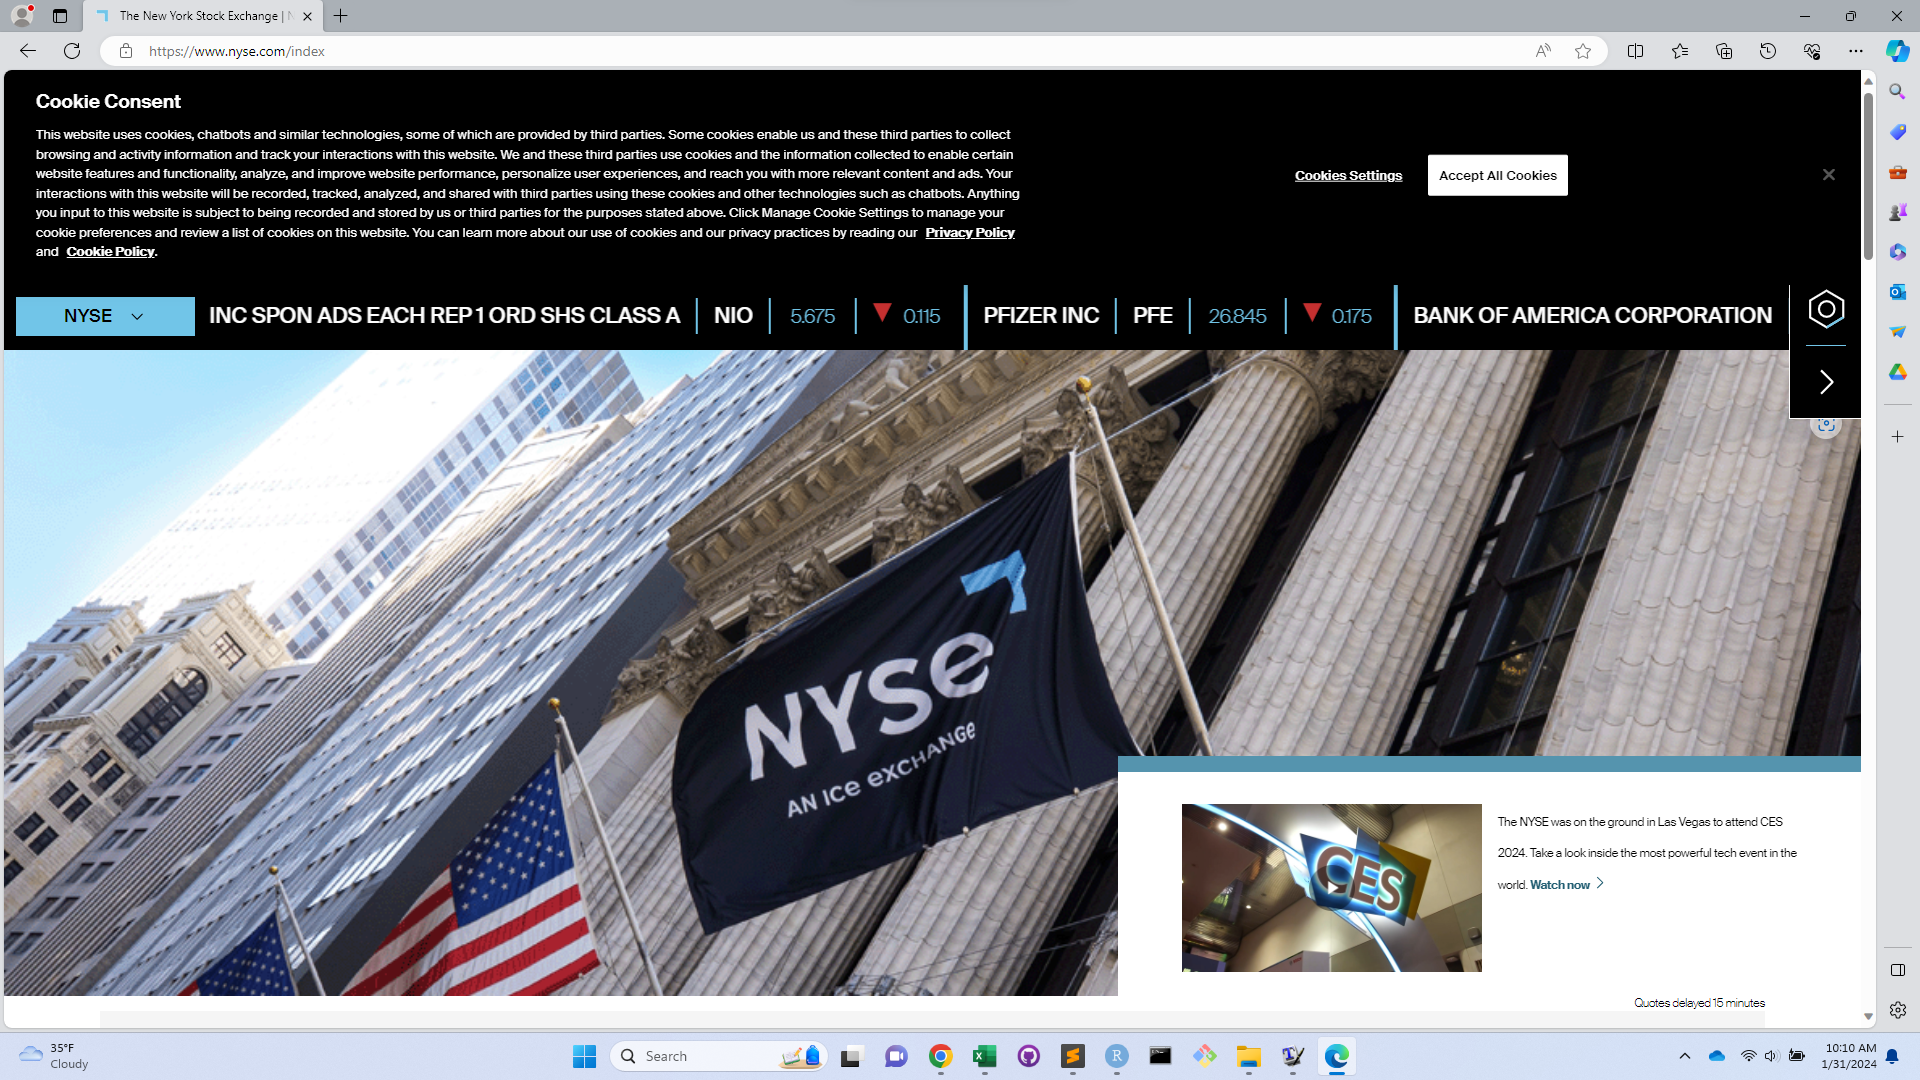
\includegraphics[clip, trim=0.0cm 0.0cm 0.0cm 0.0cm, width=1\textwidth]{Images/NYSE_Screenshot_2024_01_31_101021.png}  
    \caption{Figure {\color{franklinblue} 12}:  nyse.com Cookie Consent Banner}
    \label{fig:nyse}
\end{figure} 
\end{frame}

\begin{frame}[t]{Mobile Cookies, and First and Third Party Cookies}
``Cookies don't work on mobile'' is a commonplace belief in the digital advertising ecosystem.
However, this statement is not completely accurate which has caused much confusion in the
marketplace, as different players say different, often conflicting, things. \\
\vspace{1.5ex}
\begin{itemize}
\item A \empr{first-party cookie} is a cookie whose domain is the same as the domain of the visited website. For example, a cookie whose domain is nyse.com placed by \href{https://www.nyse.com}{http://www.nyse.com}. \\
\vspace{1.5ex}
Different mobile browsers behave differently when it comes to accepting \empr{third-party cookies}, which are cookies whose domain is different from the visited website.  For example, a cookie whose domain is nationwide.com (or \href{https://www.nationwide.com/}{Nationwide's} data management platform (DMP) or its ad server or \ldots) placed on \href{https://www.nasdaq.com/}{http://www.nasdaq.com}.
\end{itemize}
\end{frame}

\begin{frame}[t]{Nationwide Advertising on nasdaq.com}
\begin{figure}[htbp]
    \centering
    \captionsetup{justification=centering}
    
\includegraphics[clip, trim=0.0cm 0.0cm 0.0cm 0.0cm, width=1\textwidth]{Images/Nasdaq_Screenshot_2024_01_31_102418.png}  
    \caption{Figure {\color{franklinblue} 13}:  Nationwide Advertising on nasdaq.com}
    \label{fig:nyse}
\end{figure} 
\end{frame}

\begin{frame}[t]{Third Party Cookies have Been Used For Retargeting}

\begin{textblock*}{5cm}(0.2cm,1.3cm)
\begin{figure}[htbp]
  \captionsetup{justification=centering}
  
\includegraphics[height=0.8in]{Images/0SC0SETYWA.jpg}
  \caption{{\color{franklinblue} User Browser}}
\end{figure}
\end{textblock*}

\begin{textblock*}{5cm}(4.6cm,1.5cm)
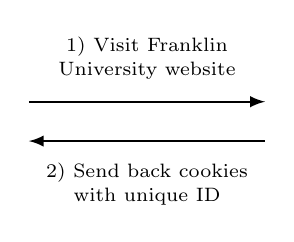
\begin{tikzpicture}
\node (a1) at (0,0.8) {\scriptsize 1) Visit Franklin}; 
\node (a2) at (0,0.5) {\scriptsize University website};
\draw[->, line width=0.3mm] (-1.5,0.1) -- (1.5,0.1);
\node (a3) at (0,-0.8) {\scriptsize 2) Send back cookies}; 
\node (a4) at (0,-1.1) {\scriptsize with unique ID};
\draw[<-, line width=0.3mm] (-1.5,-0.4) -- (1.5,-0.4);
\end{tikzpicture}
\end{textblock*}

\begin{textblock*}{5cm}(1.1cm,4.3cm)
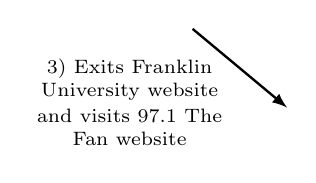
\begin{tikzpicture}
\node[align=left] (b1) at (-1.8,-0.8) {\scriptsize 3) Exits Franklin}; 
\node[align=left] (b2) at (-1.8,-1.1) {\scriptsize University website};
\node[align=left] (b3) at (-1.8,-1.4) {\scriptsize and visits 97.1 The};
\node[align=left] (b3) at (-1.8,-1.7) {\scriptsize Fan website};
\draw[->, line width=0.3mm] (-1.0,-0.3) -- (0.2,-1.3);
\end{tikzpicture}
\end{textblock*}

\begin{textblock*}{5cm}(7.5cm,1.2cm)
\begin{figure}[htbp]
  \captionsetup{justification=centering}
  
\includegraphics[height=0.8in]{Images/FU_Screenshot_ 2024_01_31_114918.png}
  \caption{{\color{franklinblue} Franklin University \\  Website}}
\end{figure}
\end{textblock*}

\begin{textblock*}{5cm}(8.5cm,4.6cm)
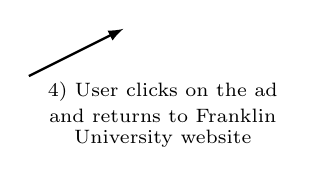
\begin{tikzpicture}
\node[align=left] (d1) at (-2.5,0.3) {\scriptsize 4) User clicks on the ad}; 
\node[align=left] (d2) at (-2.5,0) {\scriptsize and returns to Franklin};
\node[align=left] (d3) at (-2.5,-0.3) {\scriptsize University website};
\draw[->, line width=0.3mm] (-4.2,0.5) -- (-3.0,1.1);
\end{tikzpicture}
\end{textblock*}

\begin{textblock*}{5cm}(4.0cm,4.7cm)
\begin{figure}[htbp]
  \captionsetup{justification=centering}
  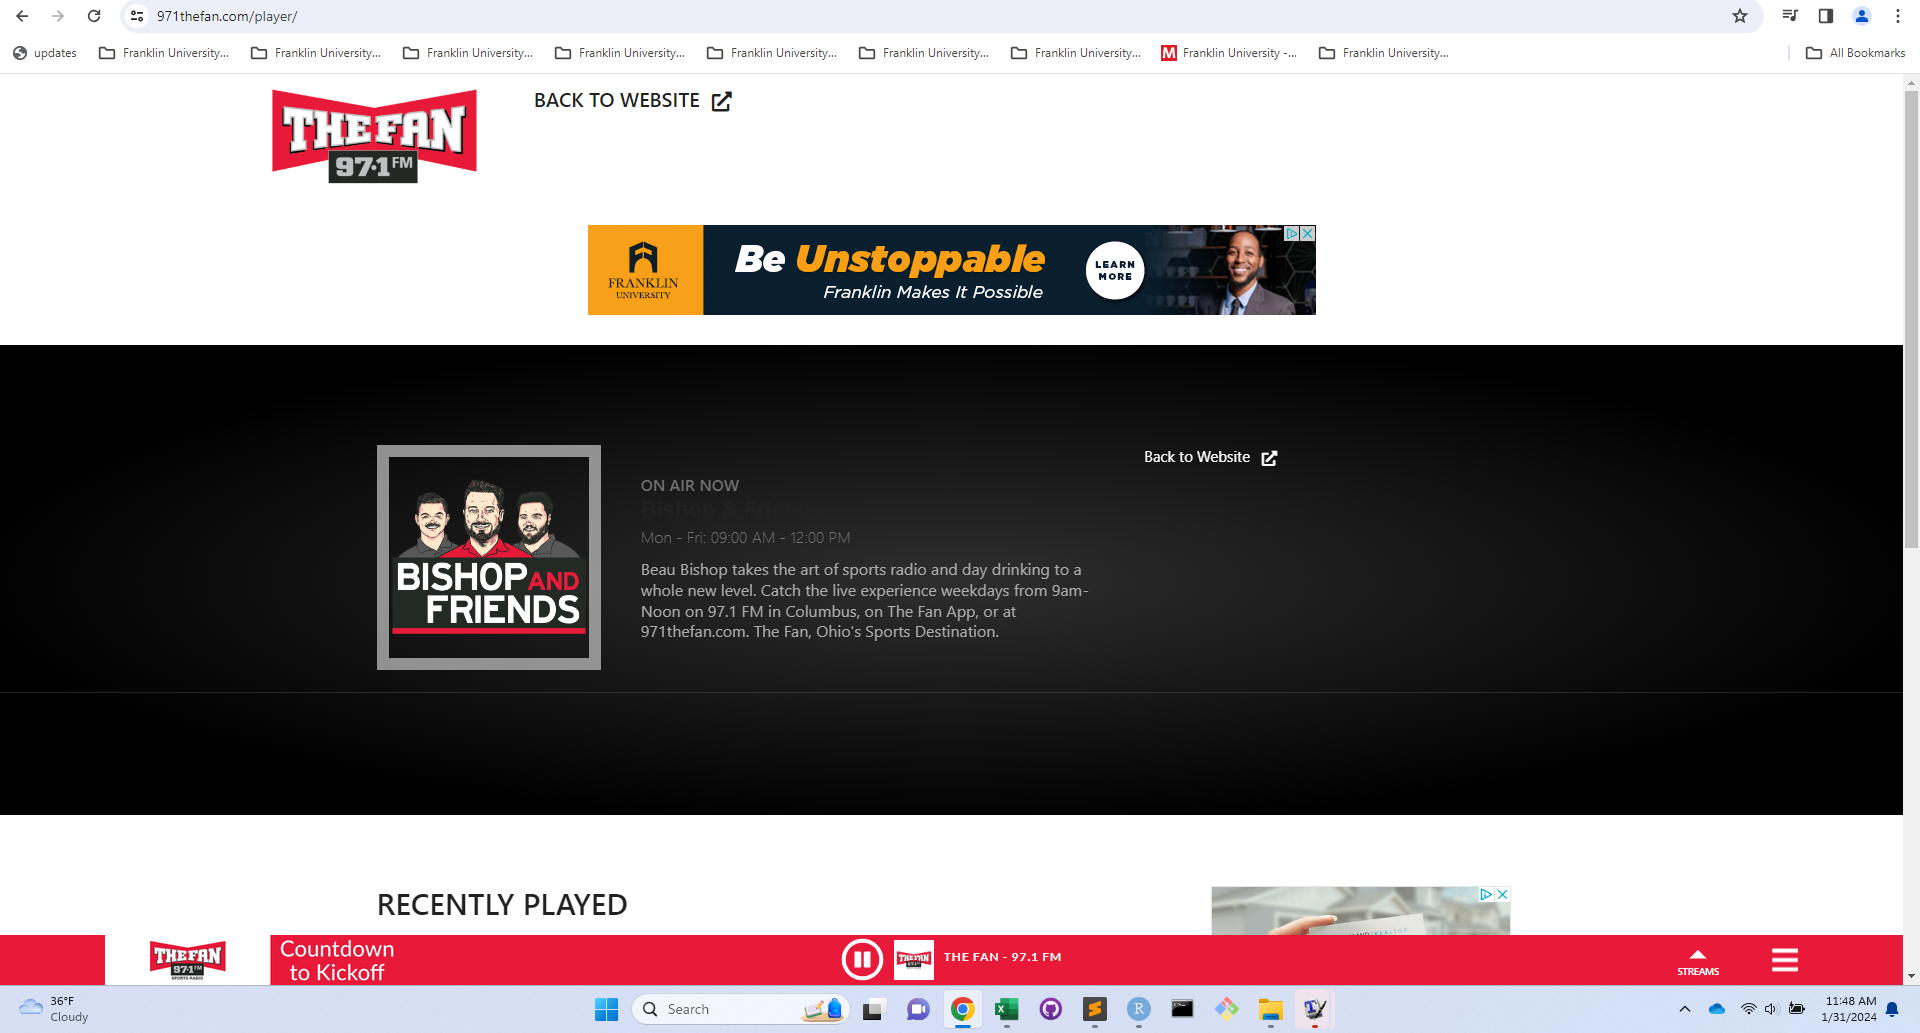
\includegraphics[height=0.8in]{Images/The_Fan_Screenshot_2024_01_31_114856.png}
  \caption{{\color{franklinblue} 97.1 The Fan Website, where a \\ Franklin University Ad is Served}}
\end{figure}
\end{textblock*}

\begin{textblock*}{5cm}(2.7cm,8.1cm)

\begin{tikzpicture}
\node (c1) at (0,0.9) {\scriptsize Cookies from Franklin University stored on user browser }; 
\node (c2) at (0,0.6) {\scriptsize  place (potentially personalized) ad on 97.1 The Fan website};
\end{tikzpicture}
\end{textblock*}
\end{frame}

\begin{frame}[t]{Mobile App Webview}
\begin{itemize}
\item In contrast to mobile browsers, mobile apps use a technology called a \empr{webview} to display online content such as a website or an ad. Cookies can be stored within a webview similar to the way they are stored in a browser setting. However, any given webview and, therefore the cookies stored in it is unique per application. \\
\vspace{1.5ex}
Mobile apps therefore cannot share cookie information with each other or with the device's mobile web browser. Each app has its own private space on the device, commonly referred to as a \underline{sandbox} environment.
\end{itemize}
\end{frame}

\begin{frame}[t]{Summarizing First and Third Party Cookies}
\small
\begin{table}[htbp]
  \centering
  \captionsetup{justification=centering}
    \begin{tabular}{|lll|}
    \toprule
   & \textbf{{\color{franklinblue} First-Party Cookies }} & \textbf{{\color{franklinblue} Third-Party Cookies}} \\
   \midrule
  {\color{franklinblue} Who Hosts} & The domain you are & Ad servers, DMPs, media  \\
  & visiting & media sites, commenting   \\
  & & aggregators, live-chat  \\
   & & pop-ups \ldots \\
     \midrule
  {\color{franklinblue} Where Tracked}  & The domain you are &  Users across many  \\
  &  visiting and in rare   & domains \\
  &  instances, other sites & \\
     \midrule
  {\color{franklinblue} Main Purpose} & Smoother site access & Enabling adware \\
     \midrule
  {\color{franklinblue} What They Do} & Remember logins,  & Retarget customers as \\
  &  preferences, shopping & they move from site \\
  &  cart items \ldots & to site \\
  \bottomrule
     \end{tabular}%
  \caption{First and Third-Party Cookie Differences}
  \label{tab:cookies}%
\end{table}%
\end{frame}

\begin{frame}[t]{Alternative Methods of Tracking}
The limitations of cookie tracking on mobile devices, Apple's \href{https://www.apple.com/newsroom/2021/01/data-privacy-day-at-apple-improving-transparency-and-empowering-users/}{app tracking transparency} (ATT) decision from a few years ago (which required mobile marketers to ask consent from users in order to track them), and Google's decision to \href{https://blog.google/products/chrome/privacy-sandbox-tracking-protection/}{eliminate third-party cookie usage in Chrome} have led to the creation of many
alternative methods of tracking. The approaches vary in methodology, implementation, and scale.  The IAB has identified \href{https://www.iab.com/wp-content/uploads/2015/08/IABDigitalSimplifiedMobileCookies.pdf}{four common solutions}. \\
\vspace{0.5ex}
\small
\begin{enumerate}
\item \underline{Client/Device Generated Identifier}: A device identifier (ID) set and/or made available by the operating system. Examples include Apple's  \href{https://developer.apple.com/documentation/adsupport/asidentifiermanager/advertisingidentifier}{Identifier for Advertisers} (IDFA) and  Google's  \href{https://support.google.com/googleplay/android-developer/answer/6048248?hl=en\#zippy=\%2Cpersistent-identifiers-including-android-id}{Android ID}.  Users may or may not be able to control or change a device-generated identifier.\footnote{For iOS 15, Apple continued to emphasize user privacy with updates to the ATT feature introduced in iOS 14. Application developers are still required to get explicit permission from users before tracking their activity across different apps and websites using IDFA.}
\end{enumerate}
\end{frame}

\begin{frame}[t]{Statistical ID and HTML5 Cookie Tracking}
\small
\begin{enumerate}
  \setcounter{enumi}{1}
\item \underline{Statistical ID}: A server-side algorithm for identifying a device or user based on the values of a combination of standard attributes passed by the device. Typical device attributes include device type, operating system, user-agent, fonts, and IP address. Those attributes change over time due to device changes or updates. \\
\vspace{1.5ex}
Statistical IDs, which are determined independently by each individual measurement organization, are inherently different than device IDs and advertising IDs in that they are not supplied directly by the device itself. 
\item \underline{HTML5 Cookie Tracking}: Also referred to as \empr{local storage} or \empr{web storage} involves storing a cookie-like file in HTML5 local storage on the device. These are similar to traditional cookies, but can only be set or retrieved when the browser is open and running.
\end{enumerate}
\end{frame}

\begin{frame}[t]{HTML5 Cookie Uses}
\small
\begin{enumerate}
\item [] Examples of HTML5 Cookie usage include: \\
\vspace{1.5ex}
\begin{itemize}
  \item E-commerce websites: Online shopping websites like \href{https://www.amazon.com/}{Amazon} and \href{https://www.ebay.com/}{eBay} use HTML5 Cookies to store user preferences, such as preferred language, currency and location settings. Additionally, these cookies store information about the items in a user's shopping cart, thus allowing users to pick up where they left off when they return to the site at a later time.
  \item Social media websites: Platforms like \href{https://www.facebook.com/}{Facebook}, \href{https://twitter.com/}{X}, and \href{https://www.linkedin.com/}{LinkedIn} use HTML5 Cookies for personalization and tracking user interactions. For instance, they may record the types of posts a user frequently interacts with to tailor their feed accordingly. Moreover, some social media websites use cookies to keep users logged in, even if they close their browser.
\end{itemize}
\end{enumerate}
\end{frame}

\begin{frame}[t]{Universal Login Tracking}
\small
\begin{enumerate}
    \setcounter{enumi}{3}
\item []
\begin{itemize}
  \item News websites: Many news sites and online publications, such as \href{https://www.nytimes.com/}{The New York Times}, \href{https://www.cnn.com/}{CNN}, and \href{https://www.bbc.com/news}{BBC}, leverage HTML5 Cookies to remember user preferences, such as their preferred news category and saved articles. Some news websites use cookies to track the number of articles a user has accessed to enforce paywalls or subscription limits.
\end{itemize}
\item \underline{Universal Login Tracking}: Requires consumers to log into different experiences using a preexisting login rather than create a unique one for that experience. This type of tracking is limited to specific vendors, but enables companies with this type of universal login to gather data across applications and devices. \\
\vspace{1.5ex}
\begin{itemize}
  \item One example is the IAB's DigiTrust ID, which has now been \href{https://iabtechlab.com/blog/digitrust-the-final-chapter/}{sunsetted}. 
  \item Another example is \href{https://www.thetradedesk.com/us/about-us/industry-initiatives/unified-id-solution-2-0}{The Trade Desk's} \href{https://unifiedid.com/}{Unified ID 2.0}. 
\end{itemize}
\end{enumerate}
\end{frame}

\begin{frame}[t]{Google's Privacy Sandbox}
In addition to the above, Google has launched the \href{https://privacysandbox.com/}{Privacy Sandbox}.  The Privacy Sandbox initiative aims to create technologies that both protect people's privacy online and give companies and developers tools to build digital businesses. The Privacy Sandbox reduces cross-site and cross-app tracking while helping to keep online content and services free. \\
\vspace{1.5ex}
\href{https://blog.google/products/chrome/privacy-sandbox-tracking-protection/}{Tracking Protection} is an element of Privacy Sandbox.  It will enable Chrome users to restrict the data that they share when visiting a website. When Tracking Protection is enabled, some websites may not load correctly;  users will have the option to temporarily re-enable third-party cookies for theses websites. \\
\vspace{1.5ex}
There is little doubt that other solutions, some expected to be favored more than others, will be proposed during the next few years.
\end{frame}

\section{References}

\begin{frame}[t,allowframebreaks]
%https://latex-beamer.com/faq/long-bibliographies-beamer/
%https://github.com/jgm/pandoc/issues/2442
\widowpenalties 1 10000
\small
\bibliography{../../Bibliography/list2}
\bibliographystyle{apalike}
\end{frame}

\end{document}